\chapter{Mesure du paramètre $\alpha^{H\tau\tau}$ dans le canal $a^{3pr}_1+\mu$}
\label{analysis}

Ce dernier chapitre constitue la suite directe du précédent avec la présentation d'une analyse complète de l'état CP du boson de Higgs et une mesure du paramètre $\alpha^{H\tau\tau}$ dans le canal $a^{3pr}_1+\mu$ grâce à la méthode du vecteur polarimétrique. 

\section{Échantillons de données}

Cette mesure est effectuée dans les données \textit{SingleMuon} enregistrées par CMS lors du Run 2 avec une luminosité intégrée totale de $137,1$ fb$^{-1}$. Le détail de la luminosité par année est donné dans le tableau \ref{lumiData}. Les échantillons de données Monte Carlo utilisés dans cette analyse regroupent tous les processus faisant intervenir la désintégration d'un boson de Higgs en une paire de leptons tau et d'autres dont la signature expérimentale est similaire à celle attendue ou pouvant mener à une erreur d'identification. Le signal est modélisé pour les trois modes de production dominants du boson de Higgs, à savoir la fusion de gluons (ggH), la fusion de bosons vecteurs (VBF) et la production associée à un boson vecteur ($VH$, $V$=$Z$,$W$) dans des échantillons sans corrélations de spin décrits dans la section \ref{CPsim}. Les processus de bruit de fond suivants sont également modélisés à travers des échantillons Monte Carlo : \\

\begin{itemize}
    \item[$\bullet$] Processus Drell-Yan $Z/\gamma^*\rightarrow ll$ associé ou non à des jets (DY + jets)
    \medskip
    \item[$\bullet$] Production d'un boson $W$ associée ou non à des jets ($W$ + jets)
    \medskip
    \item[$\bullet$] Production d'une paire $t\overline{t}$ et production single-$t/\overline{t}$
    \medskip
    \item[$\bullet$] Production d'une paire de bosons vecteurs ($VV$=$WW$, $WZ$, $ZZ$)
    \medskip
    \item[$\bullet$] Production électrofaible d'un boson $Z$ ou $W$ (EWK-W/Z)\\
\end{itemize}

La liste complète regroupant le détail des échantillons Monte Carlo utilisés dans cette analyse, le générateur employé et la section efficace associée se trouve en annexe \ref{annexA}. Les échantillons $\textit{embedded}$ décrits dans la section \ref{embed} sont également utilisés dans la description du bruit de fond associé à la désintégration $Z\rightarrow\tau\tau$.

\begin{table}[!ht]
\centering
\begin{tabular}{|c|c|}
\hline
Échantillon    & Luminosité (fb$^{-1}$) \\ \hline \hline
\textbf{2016}  & \textbf{35,9}          \\ \hline
Run2016B       & 5,79                   \\
Run2016C       & 2,57                   \\
Run2016D       & 4,25                   \\
Run2016E       & 4,01                   \\
Run2016F       & 3,10                   \\
Run2016G       & 7,54                   \\
Run2016H       & 8,61                   \\ \hline \hline
\textbf{2017}  & \textbf{41,5}          \\ \hline 
Run2017B       & 4,79                   \\
Run2017C       & 9,63                   \\
Run2017D       & 4,25                   \\
Run2017E       & 9,31                   \\
Run2017F       & 13,54                  \\ \hline \hline
\textbf{2018}  & \textbf{59,7}          \\ \hline
Run2018A       & 14,03                  \\
Run2018B       & 7,06                   \\
Run2018C       & 6,90                   \\
Run2018D       & 31,74                  \\ \hline \hline
\textbf{Total Run 2} & \textbf{137}           \\ \hline 
\end{tabular}
\caption{Luminosité intégrée par année dans les échantillons de données \textit{SingleMuon} enregistrées par CMS. Chaque année est divisée en plusieurs ères correspondant à des conditions différentes du détecteur.}
\label{lumiData}
\end{table}

\section{Reconstruction des évènements}
\label{eventreco}

Cette section vise à présenter les méthodes de reconstruction des différents objets utiles à la reconstruction de l'observable $\phi_{CP}$ dans les évènements $H\to\tau\tau$ d'état final $\mu\tau_h$. Parmi ceux-ci se trouvent les leptons ($e,\mu,\tau$), les jets, la MET, le vertex primaire, le vertex secondaire de la désintégration $\tau_h\to a_1^{3pr}$ et le paramètre d'impact du muon. Une méthode d'identification des modes de désintégration des leptons tau hadroniques, propre à cette analyse, sera également présentée. 

\subsection{Leptons}

Les électrons et muons employés dans cette analyse sont reconstruits et identifiés par l'algorithme du flux de particules selon les méthodes décrites dans les sections \ref{MuonID} et \ref{EGammaID} respectivement. Les leptons taus sont reconstruits par l'algorithme HPS décrit dans la section \ref{TauID}. La mesure de l'état CP étant directement reliée au mode de désintégration du lepton tau, un algorithme d'identification prodiguant une bonne pureté est essentiel. La principale faiblesse de l'algorithme HPS est son inaptitude à correctement identifier les pions neutres et à faussement identifier les modes de désintégrations qui en contiennent. Un BDT utilisant en entrée le mode de désintégration HPS (HPS-DM) ainsi que plusieurs variables cinématiques issues du tau hadronique est alors employé afin de redéfinir un nouveau mode de désintégration noté MVA-DM \cite{mohammadphd,mvadm}. Cet algorithme est spécifiquement optimisé dans le but d'offrir la meilleure pureté dans chaque mode de désintégration. La figure~\ref{confusionMVADM} montre les matrices de confusion du MVA-DM normalisées en ligne et en colonne, et la figure~\ref{purityMVADM} montre une comparaison de l'efficacité et de la pureté entre les HPS-DM et les MVA-DM. Les résultats montrent notamment une légère perte d'efficacité dans les états finaux à un et trois pions chargés, au profit d'une meilleure efficacité pour les états finaux avec au moins un pion neutre et d'une amélioration globale de la pureté dans tous les modes de désintégration. \\

\begin{figure}
\centering
    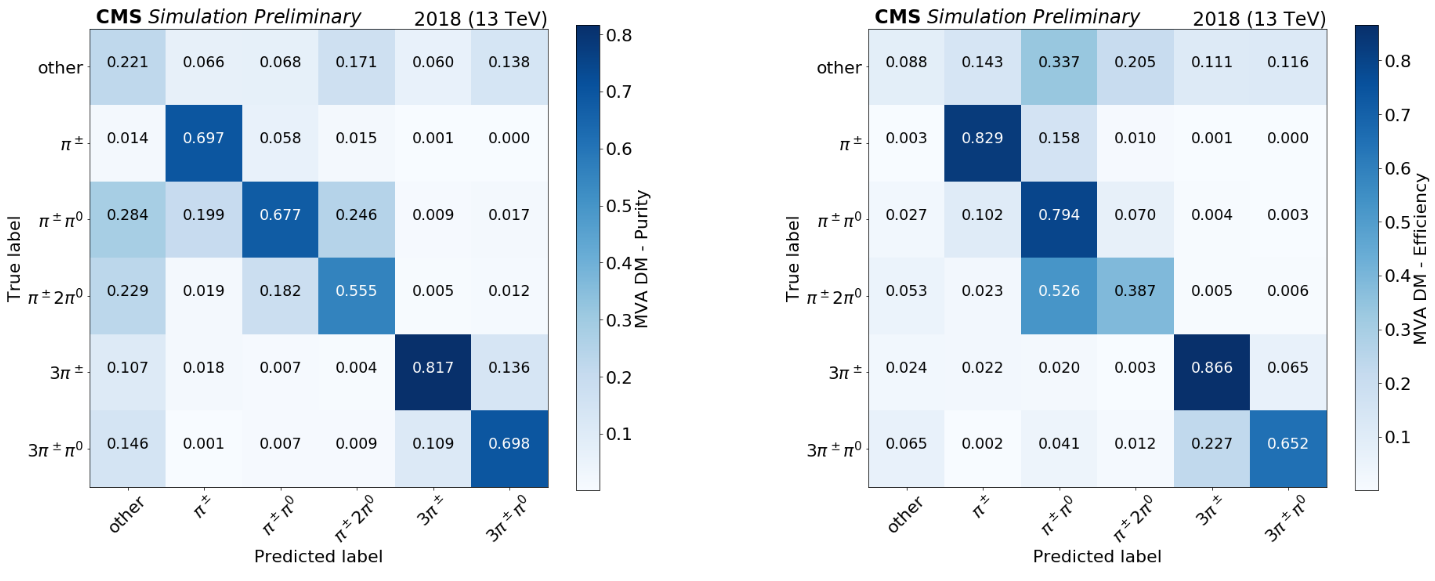
\includegraphics[scale=0.275]{Chapitre7/Images/confusionmatrixMVADM.png} 
    \caption{Matrices de confusion des MVA-DM\cite{mvadm} de pureté (gauche) et d'efficacité (droite) \cite{mvadm}.}
    \label{confusionMVADM}
\end{figure} 

\subsection{Jets}

Les jets utilisés dans cette analyse sont issus de la reconstruction effectuée par l'algorithme de regroupement anti-$k_t$ décrit dans la section \ref{JetMetID} dans des cônes de taille $R=0,4$. Afin de réduire la contribution des jets issus des interactions de l'empilement, tous les candidats du flux de particules identifiés comme hadrons chargés et qui ne sont pas associés au vertex primaire sont omis par l'algorithme de regroupement. Par ailleurs, la réponse en énergie du détecteur n'étant pas linéaire, il est difficile d'établir un lien direct entre l'énergie mesurée d'un jet à celle des particules qui le compose. Pour cette raison, plusieurs corrections sont appliquées sur l'énergie mesurée des jets à la fois sur l'échelle (JES, \textit{Jet Energy Scale}) et la résolution (JER, \textit{Jet Energy Resolution}). Après correction, les critères de sélection suivants sont appliqués : 

\begin{itemize}
    \bigskip
    \item[-] Identification \textit{Tight} des jets \cite{JetID},
    \smallskip
    \item[-] Séparation de la paire de tau sélectionnée $\Delta R>0,5$,
    \smallskip
    \item[-] $p_T>30$ GeV et $|\eta|<4,7$. 
    \bigskip
\end{itemize}

Un veto est également appliqué dans les données de 2017 sur les jets reconstruits dans la région $2,65<|\eta|<3,139$ ou dont l'impulsion transverse avant correction est inférieure à $50$ GeV afin de compenser le fort bruit présent dans les bouchons du ECAL durant cette période. Par ailleurs un jet est identifié comme issu d'un quark b (\textit{b-tag}) lorsqu'il possède les caractéristiques suivantes : 

\begin{itemize}
    \bigskip
    \item[-] $p_T>20$ GeV et $|\eta|<2,4$,
    \smallskip
    \item[-] Score \textit{deepCSV} > $0,6321$ (2016), $0,4941$ (2017), $0,4184$ (2018).
    \bigskip
\end{itemize}

\begin{figure}
\centering
    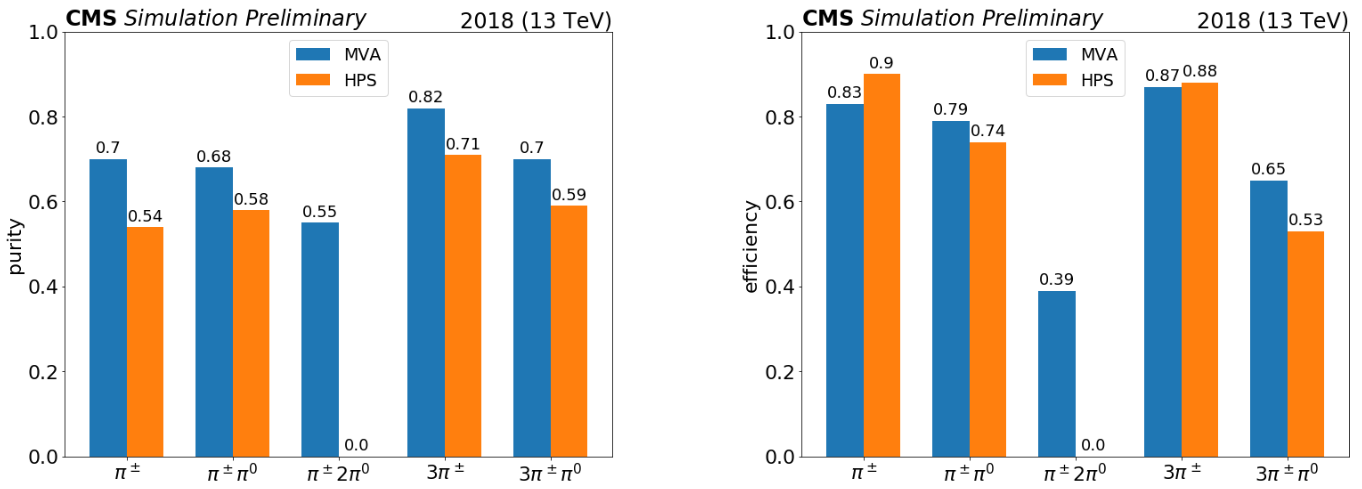
\includegraphics[scale=0.28]{Chapitre7/Images/purityvseffMVADM.png} 
    \caption{Comparaison de la pureté (gauche) et de l’efficacité (droite) par
MVA-DM (bleu) et HPS-DM (orange) \cite{mvadm}.}
    \label{purityMVADM}
\end{figure} 

\subsection{MET}
\label{MET}

La MET utilisée est reconstruite par l'algorithme PUPPI, choisi pour sa meilleure performance face à l'empilement au lieu de la MET issue du flux de particules (PF MET) \cite{puppi}. Les JEC sont ensuite propagées à la MET de la façon suivante :

$$\vv{E}^{miss,corr}_T=\vv{E}^{miss}_T-\Sigma_{jets}\bigl(\vv{p}_T^{corr}-\vv{p}_T\bigr).$$

\subsection{Vertex primaire}
\label{PVreco}

\begin{figure}
  \begin{subfigure}[b]{0.33\linewidth}
    \centering
    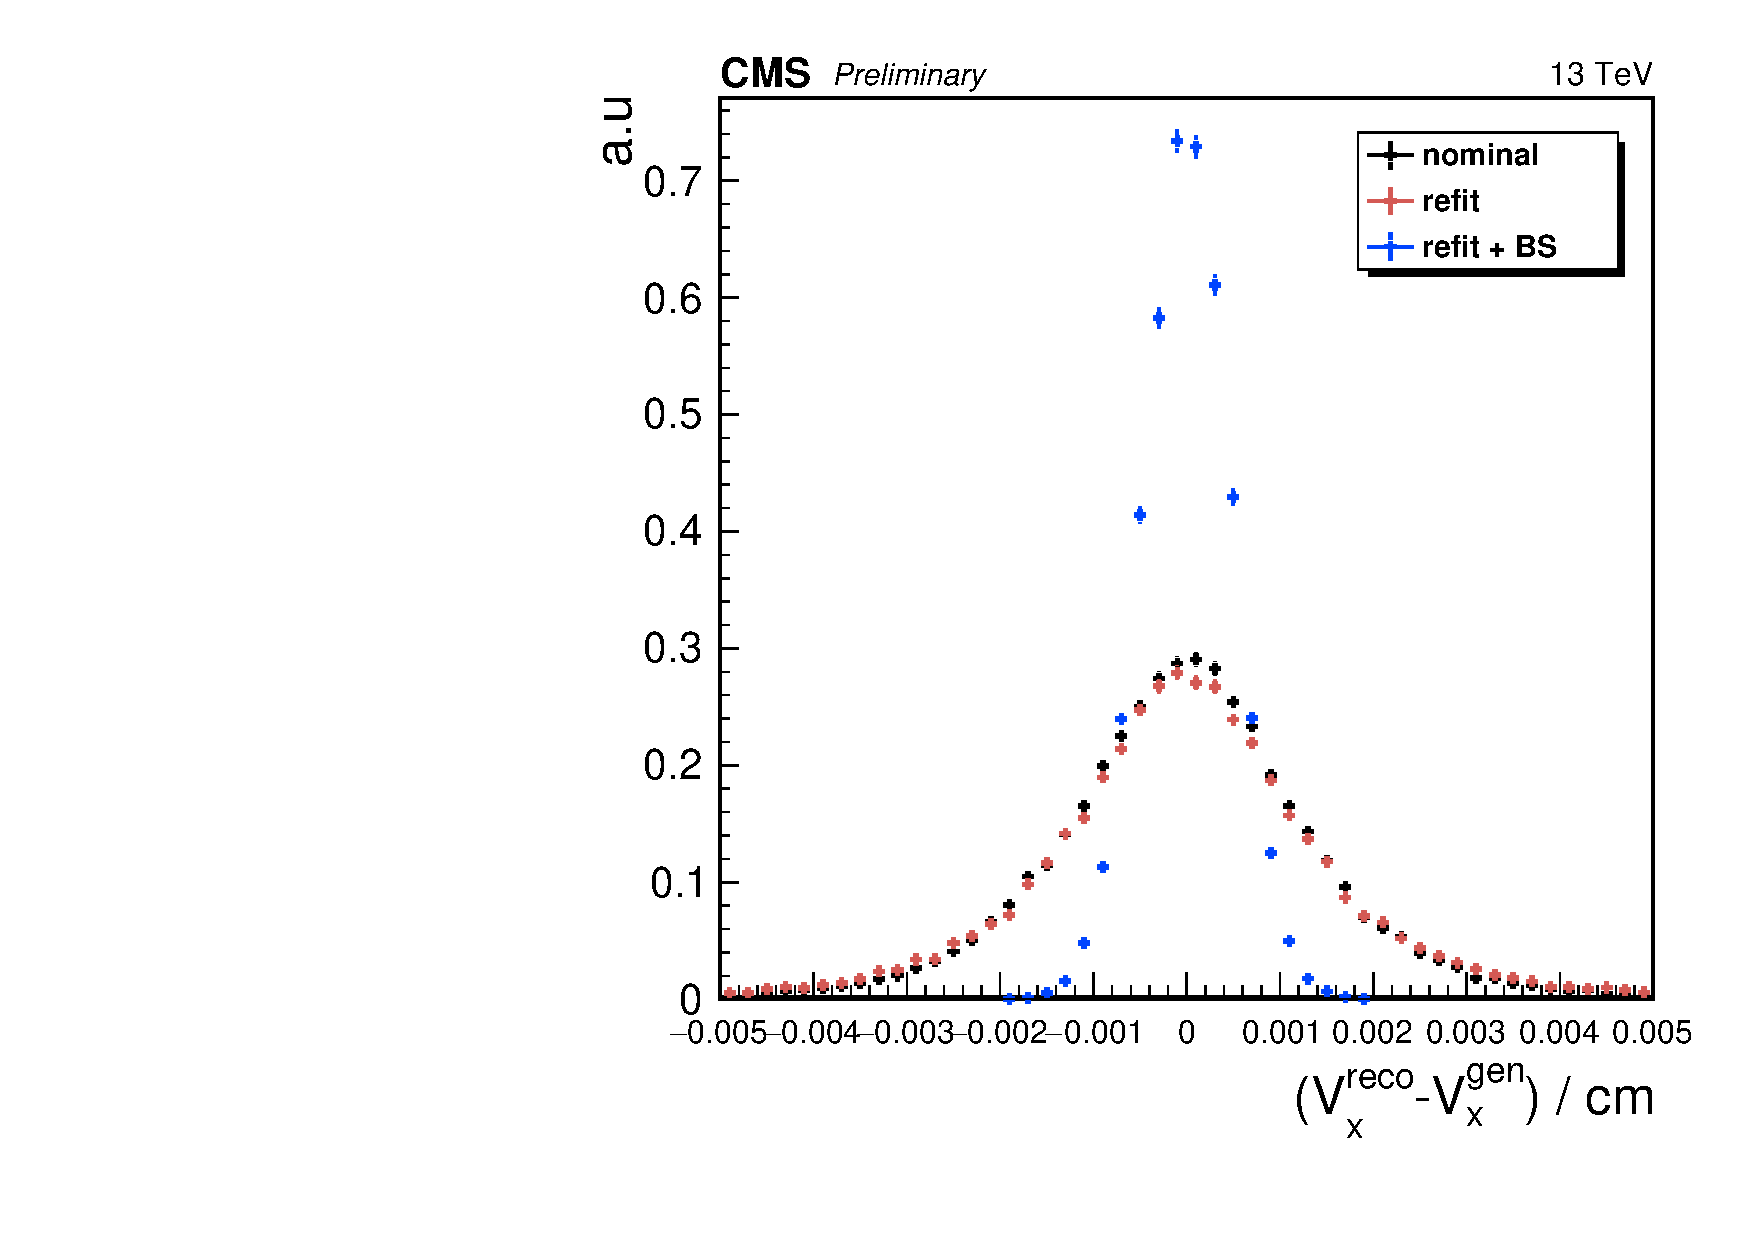
\includegraphics[width=\linewidth]{Chapitre7/Images/PVx.pdf} 
    \caption{} 
    \vspace{0.5ex}
  \end{subfigure}%% 
  \begin{subfigure}[b]{0.33\linewidth}
    \centering
    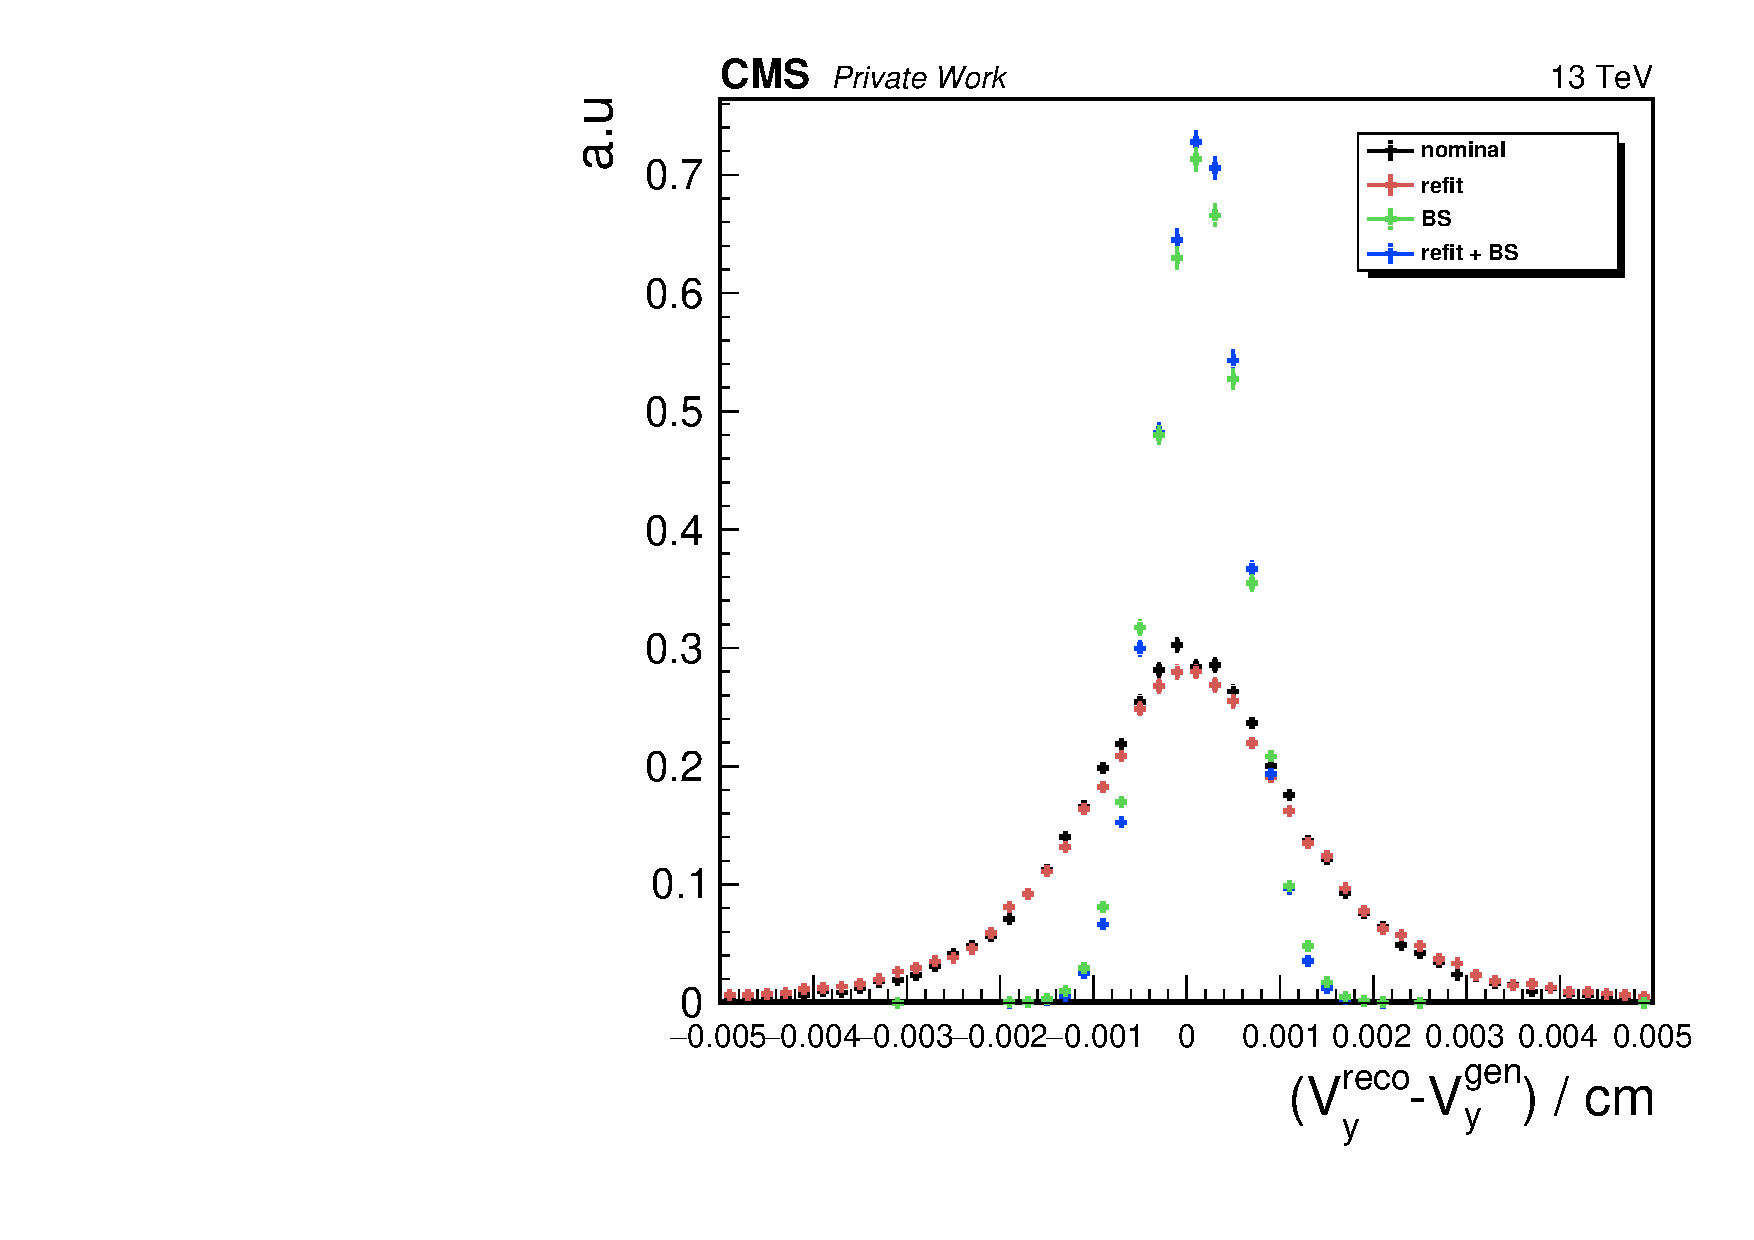
\includegraphics[width=\linewidth]{Chapitre7/Images/PVy.pdf} 
    \caption{} 
    \vspace{0.5ex}
  \end{subfigure} 
    \begin{subfigure}[b]{0.33\linewidth}
    \centering
    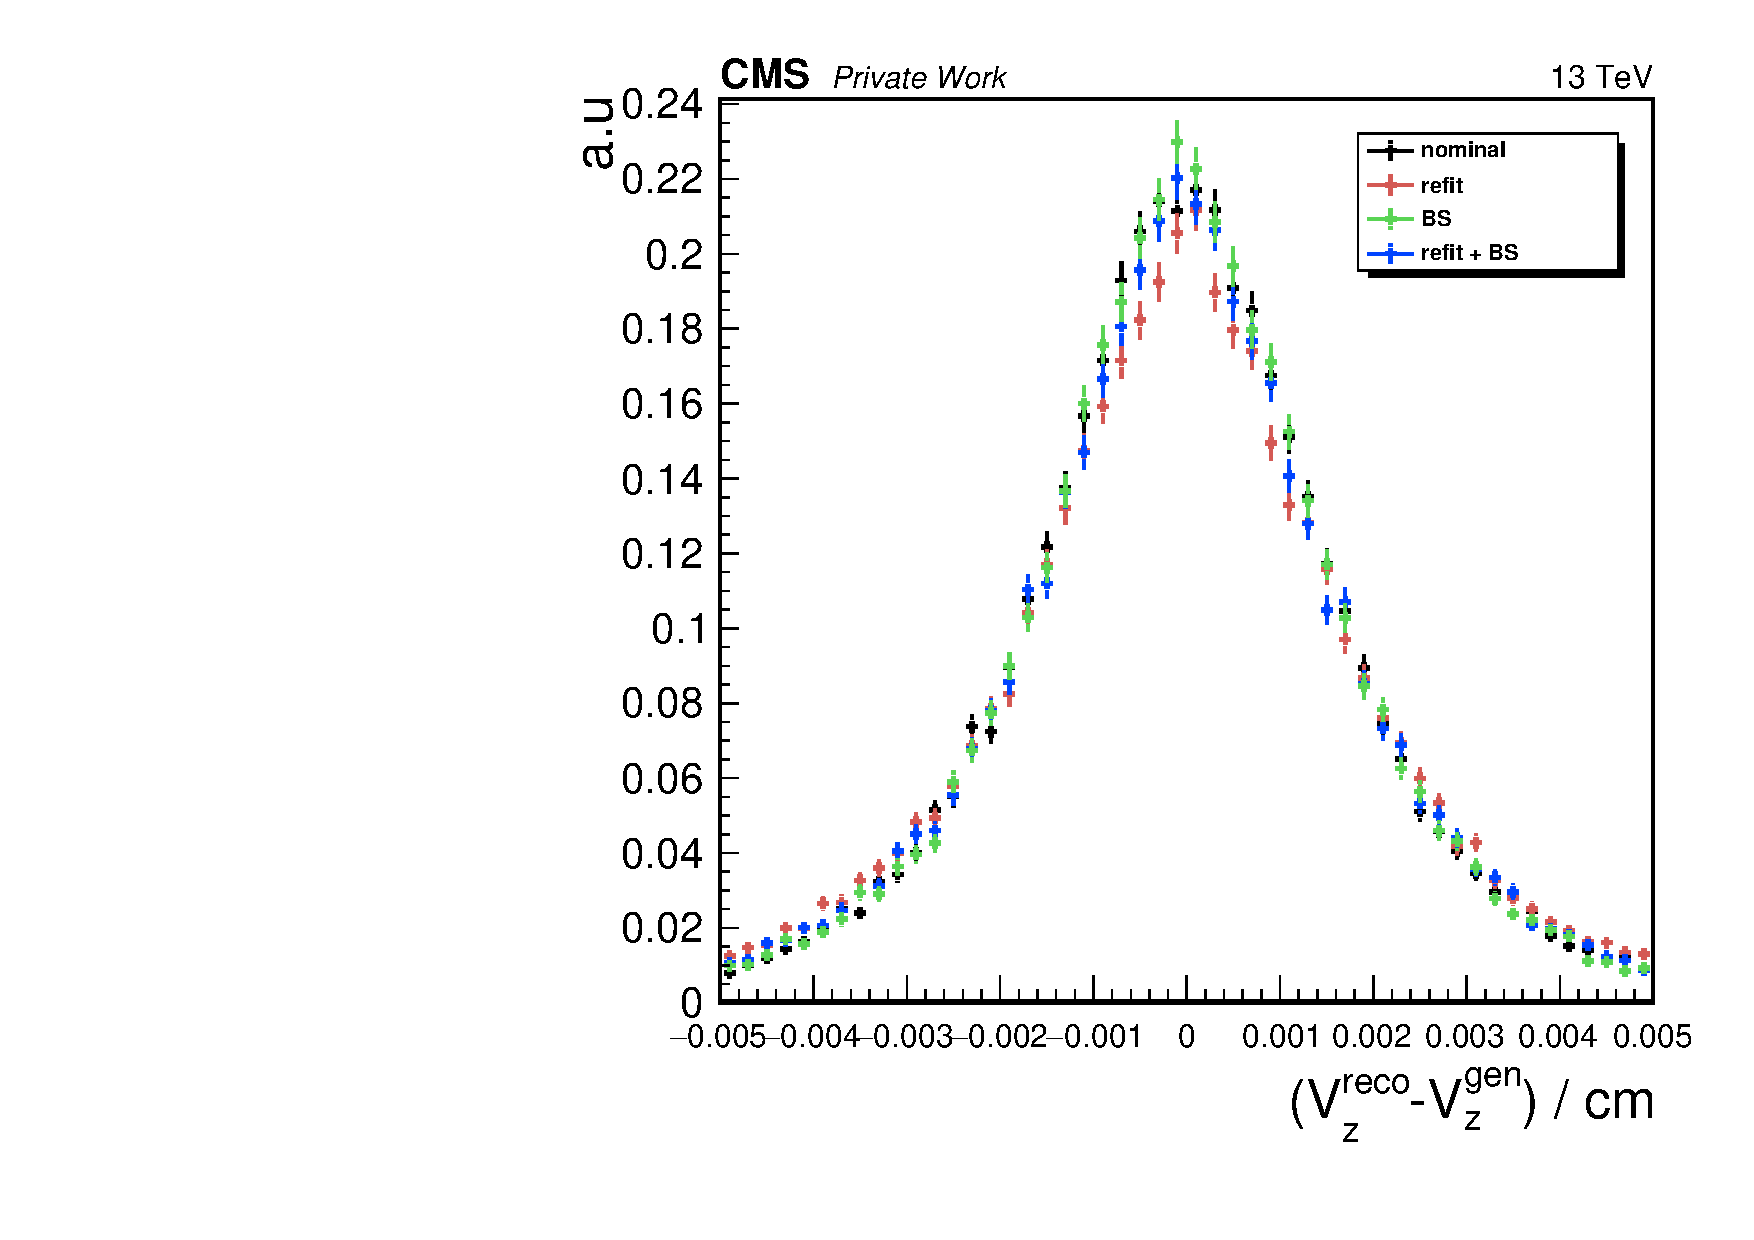
\includegraphics[width=\linewidth]{Chapitre7/Images/PVz.pdf} 
    \caption{} 
    \vspace{0.5ex}
  \end{subfigure} 
    \caption{Résolution de la reconstruction du vertex primaire pour trois niveaux de reconstruction : vertex primaire nominal (noir), vertex avec contrainte sur la position du \textit{beamspot} (vert), vertex primaire réajusté sans traces associées aux leptons tau (rouge), vertex primaire réajusté sans traces associées aux leptons tau et avec contrainte sur la position du \textit{beamspot} (bleu) également choisi pour cette analyse.}
    \label{PVreso}
\end{figure}

La reconstruction du vertex primaire (PV) permet de déterminer la position exacte de l'interaction proton-proton ayant donné lieu à un évènement et représente ainsi un enjeu crucial pour la bonne reconstruction de ce dernier. En particulier, certains éléments nécessaires à la reconstruction des observables CP tels que le paramètre d'impact ou le vecteur polarimétrique reposent sur la connaissance du vertex primaire. Deux étapes sont nécessaires durant lesquelles des ensembles de traces originaires d'un même vertex sont recherchés (regroupement), puis la meilleure estimation de la position du vertex est calculée pour chaque ensemble à partir des traces qu'il contient (ajustement). L'étape de regroupement est réalisée grâce à un algorithme basé sur le principe du \textit{deterministic annealing} (DA) \cite{annealing} visant à rechercher le minimum global d'un système possédant de nombreux degrés de liberté. Le vertex primaire est ensuite choisi en sélectionnant l'ensemble pour lequel la somme $\Sigma p_T^2$ de chaque trace est la plus grande. La position du vertex est ensuite déterminée par un ajustement des traces qui lui sont associées grâce à un algorithme nommé \textit{adaptative vertex fitter} \cite{adaptative}. Le temps de vol du lepton tau implique que ses produits de désintégration sont issus d'un vertex secondaire. Afin d'éviter un biais dans la reconstruction du vertex primaire, les traces identifiées comme provenant de la désintégration du tau sont retirées de l'ensemble lors de l'ajustement et la position du vertex est de nouveau ajustée. Une première estimation de la position du vertex est donnée par la méthode FSMW (\textit{Fraction of Sample Mode with Weights}) \cite{adaptative} avec une grande incertitude puis les traces sont ordonnées selon leur distance à cette position. Les traces sont ensuite ajoutées une par une au vertex et sa position est ajustée à chaque ajout par des filtres de Kalman. La nouvelle position du vertex est alors comparée à sa position initiale, et les traces sont pondérées selon leur compatibilité à cette nouvelle position dans le cas où l'écart avec la position initiale est significatif. Cette étape est ensuite répétée en partant de la position du vertex issue de l'itération précédente jusqu'à obtenir une position stable sur plusieurs itération, ou que le nombre maximum d'itération soit atteint. La position calculée lors de la dernière itération et l'incertitude qui lui est associée sont alors retenues. La résolution du vertex primaire peut être améliorée d'avantage en appliquant une contrainte sur la position du \textit{beamspot}, défini par le profil 3D de la zone d'interaction des faisceaux au point de collision et mesuré à partir d'une moyenne sur une grande quantité d'évènements \cite{adaptative}. Cette contrainte s'applique en choisissant la position du \textit{beamspot} comme position initiale du vertex lors de l'ajustement et remplace la méthode FSMW citée précédemment. La figure \ref{PVreso} montre que le retrait des traces associées au lepton tau avant ajustement impacte peu la résolution de reconstruction, tandis que l'ajout d'une contrainte sur la position du \textit{beamspot} l'améliore fortement selon les composantes $x$ et $y$. Le choix du vertex primaire dans le cadre de cette analyse est porté vers le vertex primaire réajusté sans traces avec une contrainte sur la position du \textit{beamspot}.

\subsection{Paramètre d'impact}
\label{IPreco}

La reconstruction tri-dimensionnelle du paramètre d'impact du muon est nécessaire pour le calcul de l'observable $\phi_{CP}$ grâce à la méthode décrite dans la section \ref{IPmethod}. Bien que la position du vertex secondaire dans le cas d'une désintégration du lepton tau en muon ou en pion n'est pas accessible, il est possible de définir le point de référence de la trace chargée comme le point de rapprochement maximal entre celle-ci et le faisceau. On notant $\vv{r}$ le vecteur entre le vertex primaire et le point de référence et $\vv{p}$ l'impulsion de la particule chargée, le paramètre d'impact $\vv{j}$ est calculé selon :

\begin{equation}
    \vv{j}=\vv{r}-\vv{r}_{\vv{p}},    
\end{equation}

avec $\vv{r}_{\vv{p}}=\frac{\vv{r}\cdot\vv{p}}{\lVert\vv{p}\rVert^2}\vv{p}$. \\

Une fois reconstruit, le paramètre d'impact est également calibré grâce à des évènements $Z\to\mu\mu$ afin de tenir compte des problèmes de simulation de cette grandeur. La signifiance $\sigma_{\vv{j}}$ du paramètre d'impact est ensuite calculée grâce à la matrice de covariance $\Sigma_{PV}$ du vertex primaire :

\begin{equation}
    \sigma_{\vv{j}}=\frac{\lVert\vv{j}\rVert}{\hat{j}\cdot(\Sigma_{PV}\times\hat{j})},
\end{equation}
où $\hat{j}$ est le paramètre d'impact unitaire. La figure \ref{IPxyz} montre la distribution de chaque coordonnée cartésienne du paramètre d'impact reconstruit et la distribution de sa signifiance. Le calcul de $\sigma_{\vv{j}}$ permet d'identifier les évènements où le paramètre d'impact est mal reconstruit et ainsi les évènements $\tau_h\mu$ où $\sigma_{\vv{j}}<1,5$ pour le muon sont rejetés.


\begin{figure}[!ht]
\begin{subfigure}[b]{\linewidth}
    \centering
    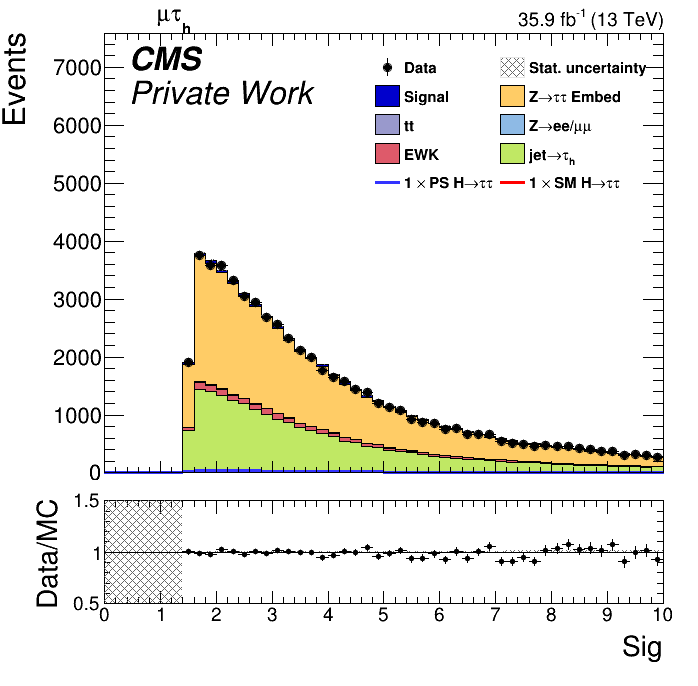
\includegraphics[scale=0.3]{Chapitre7/Images/MuonIPsig.png} 
    \caption{} 
    \vspace{0.5ex}
  \end{subfigure}
  \begin{subfigure}[b]{0.33\linewidth}
    \centering
    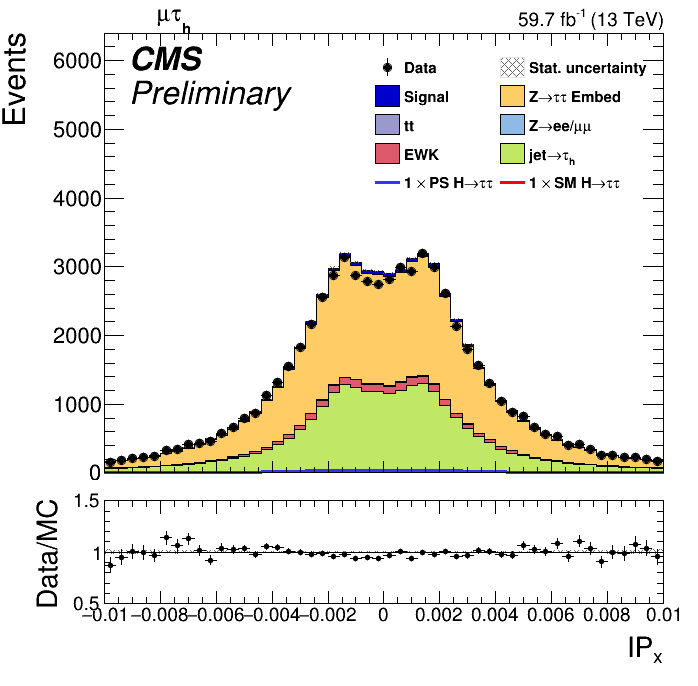
\includegraphics[width=\linewidth]{Chapitre7/Images/MuonIPx.png} 
    \caption{} 
    \vspace{0.5ex}
  \end{subfigure}%% 
  \begin{subfigure}[b]{0.33\linewidth}
    \centering
    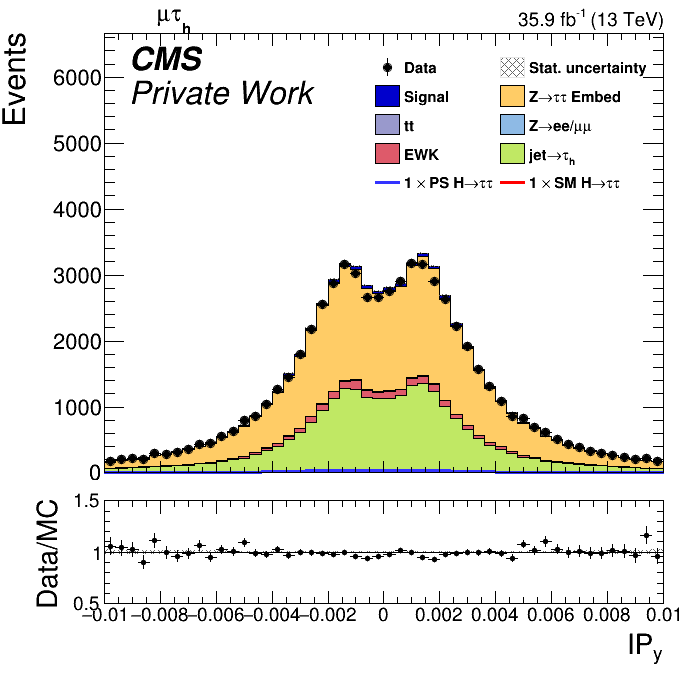
\includegraphics[width=\linewidth]{Chapitre7/Images/MuonIPy.png} 
    \caption{} 
    \vspace{0.5ex}
  \end{subfigure} 
    \begin{subfigure}[b]{0.33\linewidth}
    \centering
    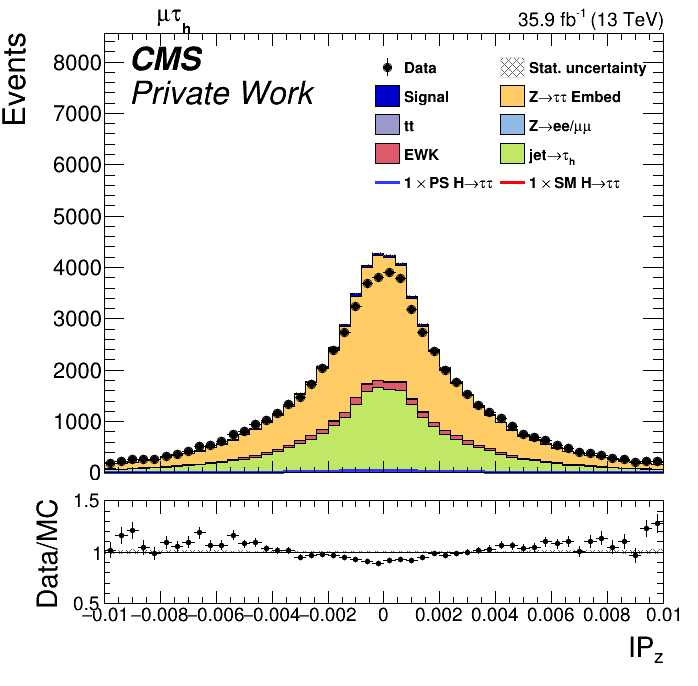
\includegraphics[width=\linewidth]{Chapitre7/Images/MuonIPz.png} 
    \caption{} 
    \vspace{0.5ex}
  \end{subfigure}
    \caption{Distribution de la signifiance (a) et des trois coordonnées cartésiennes $x$ (b), $y$ (c) et $z$ (d) du paramètre d'impact du muon reconstruit et calibré dans les données 2018.}
    \label{IPxyz}
\end{figure}


\section{Système de déclenchement}

Un évènement est sélectionné lorsqu'il active le système de déclenchement du détecteur selon l'un des chemins listés dans les tableaux \ref{trg16} (2016), \ref{trg17} (2017) et \ref{trg18} (2018). Dans le canal $\mu\tau_h$, cette sélection requière la présence d'au moins un muon (\textit{SingleMuonX}), ou la présence d'un tau hadronique associée à celle d'un muon (\textit{MuonXTauY}), où X et Y représentent le seuil de déclenchement en impulsion transverse du muon et du tau respectivement. 

%%%%TRIGGER 2016%%%%
\begin{table}[]
\resizebox{14.1cm}{!}{
\begin{tabular}{|llcl|}
\hline
\multicolumn{4}{|c|}{$\mu\tau_h$ channel} \\ \hline
\multicolumn{1}{|l|}{HLT Path}                                                                                       & \multicolumn{1}{l|}{L1 seed}                                                                        & \multicolumn{2}{c|}{Muon filter(s) to match}   \\ \hline
\multicolumn{1}{|l|}{\begin{tabular}[c]{@{}l@{}}HLT\_IsoMu22\_v\\ HLT\_IsoMu22\_eta2p1\_v\end{tabular}}              & \multicolumn{1}{l|}{\begin{tabular}[c]{@{}l@{}}L1\_SingleMu20\\ L1\_SingleMu20er\end{tabular}}      & \multicolumn{2}{c|}{\begin{tabular}[c]{@{}c@{}}hltL3crIsoL1sMu20L1f0L2f10QL3f22QL3trkIsoFiltered0p09\\ hltL3crIsoL1sSingleMu20erL1f0L2f10QL3f22QL3trkIsoFiltered0p09\end{tabular}}                                                                                                                                                 \\ \hline
\multicolumn{1}{|l|}{\begin{tabular}[c]{@{}l@{}}HLT\_IsoTkMu22\_v\\ HLT\_IsoTkMu22\_eta2p1\_v\end{tabular}}          & \multicolumn{1}{l|}{\begin{tabular}[c]{@{}l@{}}L1\_SingleMu20 \\ L1\_SingleMu20er\end{tabular}}   & \multicolumn{2}{c|}{\begin{tabular}[c]{@{}c@{}}hltL3fL1sMu20L1f0Tkf22QL3trkIsoFiltered0p09\\ hltL3fL1sMu20erL1f0Tkf22QL3trkIsoFiltered0p09\end{tabular}}    \\ \hline
\multicolumn{2}{|l|}{}        & \multicolumn{1}{c|}{Muon filter(s) to match}        & \multicolumn{1}{c|}{Tau filter(s) to match}      \\ \hline
\multicolumn{1}{|l|}{\begin{tabular}[c]{@{}l@{}}HLT\_IsoMu19\_eta2p1\_LooseIso-\\ PFTau20\_v\end{tabular}}           & \multicolumn{1}{l|}{L1\_Mu18er\_Tau20er}                                                            & \multicolumn{1}{l|}{\begin{tabular}[c]{@{}l@{}}hltL3crIsoL1sMu18erTauJet20er-\\ L1f0L2f10QL3f19QL3trkIsoFiltered0p09,\\ hltOverlapFilterIsoMu19LooseIsoPFTau20\end{tabular}}                      & \begin{tabular}[c]{@{}l@{}}hltPFTau20TrackLooseIsoAgainstMuon,\\ hltOverlapFilterIsoMu19LooseIsoPFTau20\end{tabular}           \\ \hline
\multicolumn{1}{|l|}{\begin{tabular}[c]{@{}l@{}}HLT\_IsoMu19\_eta2p1\_LooseIso-\\ PFTau20\_SingleL1\_v\end{tabular}} & \multicolumn{1}{l|}{\begin{tabular}[c]{@{}l@{}}L1\_SingleMu18er OR\\ L1\_SingleMu20er\end{tabular}} & \multicolumn{1}{l|}{\begin{tabular}[c]{@{}l@{}}hltL3crIsoL1sSingleMu18erIorSingleMu20er-\\ L1f0L2f10QL3f19QL3trkIsoFiltered0p09,\\ hltOverlapFilterSingleIsoMu19LooseIso-\\ PFTau20\end{tabular}} & \begin{tabular}[c]{@{}l@{}}hltPFTau20TrackLooseIsoAgainstMuon,\\ hltOverlapFilterSingleIsoMu19LooseIso-\\ PFTau20\end{tabular} \\ \hline
\end{tabular}
}
\caption{Liste des chemins HLT et des filtres associés pour les données 2016 dans le canal $\mu\tau_h$.}
\label{trg16}
\end{table}
%%%TRIGGER 2017%%%%%%
\begin{table}[]
\resizebox{14.1cm}{!}{
\begin{tabular}{|llll|}
\hline
\multicolumn{4}{|c|}{$\mu\tau_h$ channel}                                                                                                                              \\ \hline
\multicolumn{1}{|l|}{HLT Path}    & \multicolumn{1}{l|}{L1 seed}                                                           & \multicolumn{2}{c|}{Muon filter(s) to match}                                                                 \\ \hline 
\multicolumn{1}{|l|}{HLT\_IsoMu\_24\_v}                                                                                              & \multicolumn{1}{l|}{L1\_SingleMu22}                                                                                            & \multicolumn{2}{l|}{hltL3crIsoL1sSingleMu22L1f0L2f10QL3f24QL3trkIsoFiltered0p07}  \\ \hline
\multicolumn{1}{|l|}{HLT\_IsoMu27\_v}                                                                                                & \multicolumn{1}{l|}{\begin{tabular}[c]{@{}l@{}}L1\_SingleMu22 \quad OR \\ L1\_SingleMu25\end{tabular}} & \multicolumn{2}{l|}{hltL3crIsoL1sMu22Or25L1f0L2f10QL3f27QL3trkIsoFiltered0p07}                                                                                                           \\ \hline
\multicolumn{2}{|l|}{}     & \multicolumn{1}{c|}{Muon filter(s) to match}                                           & \multicolumn{1}{c|}{Tau filter(s) to match}      \\ \hline
\multicolumn{4}{|c|}{Data and MC}      \\ \hline
\multicolumn{1}{|l|}{\begin{tabular}[c]{@{}l@{}}HLT\_IsoMu20\_eta2p1\_\\ LooseChargedIsoPFTau27\\ \_eta2p1\_CrossL1\_v\end{tabular}} & \multicolumn{1}{l|}{L1\_Mu18er2p1\_Tau24er2p1}                                                                                 & \multicolumn{1}{l|}{\begin{tabular}[c]{@{}l@{}}hltL3crIsoL1sMu18erTau24erIorMu20er\_\\ Tau24erL1f0L2f10QL3f20QL3trkIsoFiltered\_\\ 0p07, hltOverlapFilterIsoMu20LooseCharged\_\\ IsoPFTau27L1Seeded\end{tabular}} & \begin{tabular}[c]{@{}l@{}}hltSelectedPFTau27LooseChargedIsolation\_\\ AgainstMuonL1HLTMatched,\\ hltOverlapFilterIsoMu20LooseChargedIso\_\\ PFTau27L1Seeded\end{tabular} \\ \hline
\multicolumn{4}{|c|}{Embedded}      \\ \hline
\multicolumn{1}{|l|}{\begin{tabular}[c]{@{}l@{}}HLT\_IsoMu20\_eta2p1\_\\ LooseChargedIsoPFTau27\\ \_eta2p1\_CrossL1\_v\end{tabular}} & \multicolumn{1}{l|}{L1\_Mu18er2p1\_Tau24er2p1}                                                                                 & \multicolumn{1}{l|}{\begin{tabular}[c]{@{}l@{}}hltL3crIsoL1sMu18erTau24erIorMu20er-\\ Tau24erL1f0L2f10QL3f20QL3trkIsoFiltered0p07\end{tabular}} & \begin{tabular}[c]{@{}l@{}}hltL1sMu18erTau24erIorMu20erTau24er\end{tabular} \\ \hline
\end{tabular}
}
\caption{Liste des chemins HLT et des filtres associés pour les données 2017 dans le canal $\mu\tau_h$.}
\label{trg17}
\end{table}
%%%TRIGGER 2018%%%%
\begin{table}[]
\centering
\resizebox{14.1cm}{!}{
%\hspace*{-5cm}
\begin{tabular}{|llcl|}
\hline
\multicolumn{4}{|c|}{$\mu\tau_h$ channel}   \\ \hline
\multicolumn{1}{|l|}{HLT Path}    & \multicolumn{1}{l|}{L1 seed}      & \multicolumn{2}{c|}{Muon filter(s) to match}       \\ \hline
\multicolumn{1}{|l|}{HLT\_IsoMu24\_v}                     & \multicolumn{1}{l|}{L1\_SingleMu22}      & \multicolumn{2}{c|}{hltL3crIsoL1sSingleMu22L1f0L2f10QL3f24QL3trkIsoFiltered0p07}       \\ \hline
\multicolumn{1}{|l|}{HLT\_IsoMu27\_v}               & \multicolumn{1}{l|}{\begin{tabular}[c]{@{}l@{}}L1\_SingleMu22 OR\\ L1\_SingleMu25\end{tabular}} & \multicolumn{2}{c|}{hltL3crIsoL1sMu22Or25L1f0L2f10QL3f27QL3trkIsoFiltered0p07}                                                   \\ \hline
\multicolumn{2}{|l|}{}                                                                    & \multicolumn{1}{c|}{Muon filter(s) to match}                         & \multicolumn{1}{c|}{Tau filter(s) to match}          \\ \hline
\multicolumn{4}{|c|}{Run \textless 315974}     \\ \hline
\multicolumn{1}{|l|}{\begin{tabular}[c]{@{}l@{}}HLT\_IsoMu20\_eta2p1\_\\ LooseChargedIsoPFTau27\_\\ eta2p1\_CrossL1\_v\end{tabular}}             & \multicolumn{1}{l|}{L1\_Mu18er2p1\_Tau24er2p1}                                                  & \multicolumn{1}{l|}{\begin{tabular}[c]{@{}l@{}}hltL3crIsoL1sMu18erTau24erIorMu20er-\\ Tau24erL1f0L2f10QL3f20QL3trkIsoFiltered-\\ 0p07, hltOverlapFilterIsoMu20LooseCharged-\\ IsoPFTau27L1Seeded\end{tabular}}       & \begin{tabular}[c]{@{}l@{}}hltSelectedPFTau27LooseChargedIsolation-\\ AgainstMuonL1HLTMatched,\\ hltOverlapFilterIsoMu20LooseChargedIso-\\ PFTau27L1Seeded\end{tabular}                                           \\ \hline
\multicolumn{4}{|c|}{315974 $\leq$ Run $\leq$ 317509}    \\ \hline
\multicolumn{1}{|l|}{\begin{tabular}[c]{@{}l@{}}HLT\_IsoMu20\_eta2p1\_\\ LooseChargedIsoPFTau27\_\\ eta2p1\_CrossL1\_v\end{tabular}}    & \multicolumn{1}{l|}{L1\_Mu18er2p1\_Tau24er2p1}         & \multicolumn{1}{l|}{\begin{tabular}[c]{@{}l@{}}hltL3crIsoBigORMu18erTauXXer2p1L1f0-\\ L2f10QL3f20QL3trkIsoFiltered0p07,\\ hltOverlapFilterIsoMu20LooseCharged-\\ IsoPFTau27L1Seeded\end{tabular}}                    & \begin{tabular}[c]{@{}l@{}}hltSelectedPFTau27LooseChargedIsolation-\\ AgainstMuonL1HLTMatched,\\ hltOverlapFilterIsoMu20LooseCharged-\\ IsoPFTau27L1Seeded\end{tabular}                        \\ \hline
\multicolumn{4}{|c|}{Run \textgreater 317509 and MC}      \\ \hline
\multicolumn{1}{|l|}{\begin{tabular}[c]{@{}l@{}}HLT\_IsoMu20\_eta2p1\_\\ LooseChargedIsoPFTauHPS27\_\\ eta2p1\_CrossL1\_v\end{tabular}} & \multicolumn{1}{l|}{L1\_Mu18er2p1\_Tau24er2p1}                                                  & \multicolumn{1}{l|}{\begin{tabular}[c]{@{}l@{}}hltL3crIsoBigORMu18erTauXXer2p1L1f0-\\ L2f10QL3f20QL3trkIsoFiltered0p07,\\ hltHpsOverlapFilterIsoMu20LooseCharged-\\ IsoTightOOSCPhotonsPFTau27L1Seeded\end{tabular}} & \begin{tabular}[c]{@{}l@{}}hltHpsSelectedPFTau27LooseCharged-\\ IsolationTightOOSCPhotonsAgainst-\\ MuonL1HLTMatched,\\ hltHpsOverlapFilterIsoMu20LooseCharged-\\ IsoTightOOSCPhotonsPFTau27L1Seeded\end{tabular} \\ \hline
\multicolumn{4}{|c|}{Embedded}     \\ \hline
\multicolumn{1}{|l|}{\begin{tabular}[c]{@{}l@{}}HLT\_IsoMu20\_eta2p1\_\\ LooseChargedIsoPFTauHPS27\_\\ eta2p1\_CrossL1\_v\end{tabular}} & \multicolumn{1}{l|}{L1\_Mu18er2p1\_Tau24er2p1}                                                  & \multicolumn{1}{l|}{\begin{tabular}[c]{@{}l@{}}hltL3crIsoBigORMu18erTauXXer2p1L1f0-\\L2f10QL3f20QL3trkIsoFiltered0p07\end{tabular}} & \begin{tabular}[c]{@{}l@{}}hltL1sBigORMu18erTauXXer2p1\\ \end{tabular} \\ \hline
\end{tabular}
}
\caption{Liste des chemins HLT et des filtres associés pour les données 2018 dans le canal $\mu\tau_h$.}
\label{trg18}
\end{table}

\section{Sélection des évènements}

Cette section est dédiée à la description des critères de sélection des évènements. Les coupures communes à tous les canaux seront présentées dans un premier temps, puis la sélection des évènements dans le canal $\tau\tau\rightarrow\mu+\tau_h$ dans un second temps.

\subsubsection{\ding{95} Filtres appliqués à la MET}

Les évènements doivent passer chacun des filtres suivants afin d'être sélectionnés :

\begin{itemize}
\bigskip
    \item[-] \textit{Primary vertex filter} (données et MC),
        \smallskip
    \item[-] \textit{Beam halo filter super tight} (données et MC),
        \smallskip
    \item[-] \textit{HBHE noise filter} (données et MC),
        \smallskip
    \item[-] \textit{HBHEiso noise filter} (données et MC),
        \smallskip
    \item[-] \textit{eebadSC noise filter} (données),
        \smallskip
    \item[-] \textit{ECAL TP filter} (données et MC),
        \smallskip
    \item[-] \textit{badMuon filter} (données et MC),
        \smallskip
    \item[-] \textit{ECAL bad calibration filter} (données et MC, 2017 et 2018).
    \bigskip
\end{itemize}

\subsubsection{\ding{95} Exclusion des leptons supplémentaires}

Les évènements contenant un lepton supplémentaire aux deux leptons requis par le système de déclenchement sont écartés si ce dernier possède les caractéristiques suivantes : \\


\textbf{Électrons} :

\begin{itemize}
\bigskip
    \item[-] $p_{T}>10$ GeV et $|\eta|<2,5$,
        \smallskip
    \item[-] $d_z<0,2$ cm et $d_{xy}<0,045$ cm,
        \smallskip
    \item[-] Identifié au point de fonctionnement à 90\% 
    d'efficacité de l'électron ID sans critère d'isolement (entraînement Fall17-V2),
        \smallskip
    \item[-] N'est pas issu d'une conversion (\textit{passConversionVeto}),
        \smallskip
    \item[-] Nombre d'impacts internes de la trace GSF manquants $\leq 1$, 
        \smallskip
    \item[-] Isolement relatif < $0,3$ dans un cône de taille $R=0,3$. 
    \bigskip
\end{itemize}

\textbf{Muons} :

\begin{itemize}
\bigskip
    \item[-] $p_{T}>10$ GeV et $|\eta|<2,4$,
        \smallskip
    \item[-] $d_z<0,2$ cm et $d_{xy}<0,045$ cm,
        \smallskip
    \item[-] Identifié au point de fonctionnement \textit{Medium} du muon ID,
        \smallskip
    \item[-] Isolement relatif < $0,3$ dans un cône de taille $R=0,4$. 
    \bigskip
\end{itemize}

\subsubsection{\ding{95} Exclusion des paires de leptons}

Les évènements contenant une paire de leptons sont écartés si ces derniers ont une distance relative $\Delta R<0,15$ et possèdent les caractéristiques suivantes : \\

\textbf{Di-électrons} :

\begin{itemize}
\bigskip
    \item[-] $p_{T}>15$ GeV et $|\eta|<2,5$,
        \smallskip
    \item[-] $d_z<0,2$ cm et $d_{xy}<0,045$ cm,
        \smallskip
    \item[-] Identifiés au point de fonctionnement à 90\% d'efficacité de l'électron ID sans critère d'isolement (entraînement Fall17-V2),
        \smallskip
    \item[-] Isolement relatif < $0,3$ avec correction de la position de la zone d'interaction du faisceau (\textit{beamspot}) dans un cône de taille $R=0,3$. 
    \bigskip
\end{itemize}

\textbf{Di-muons} :

\begin{itemize}
\bigskip
    \item[-] $p_{T}>15$ GeV et $|\eta|<2,4$,
        \smallskip
    \item[-] $d_z<0,2$ cm et $d_{xy}<0,045$ cm,
        \smallskip
    \item[-] Muons de types \textit{tracker} et \textit{global},
        \smallskip
    \item[-] Muons issus du flux de particules (PF muons),
        \smallskip
    \item[-] Isolement relatif < $0,3$ dans un cône de taille $R=0,4$. 
    \bigskip
\end{itemize}

\subsubsection{\ding{95} Coupures dans le canal $\mu\tau_h$}

Un évènement est pré-sélectionné si au moins une paire contenant un muon et un tau hadronique est trouvée et si chaque candidat possède les caractéristiques suivantes : \\

\textbf{Muon} :

\begin{itemize}
\bigskip
    \item[-] $p_{T}>20$ GeV et $|\eta|<2,4$,
        \smallskip
    \item[-] $d_z<0,2$ cm et $d_{xy}<0,045$ cm,
        \smallskip
    \item[-] Identifié au point de fonctionnement \textit{Medium} du Muon ID,
        \smallskip
    \item[-] Isolement relatif < $0,15$. 
    \bigskip
\end{itemize}

\textbf{Tau hadronique} :

\begin{itemize}
\bigskip
    \item[-] $p_{T}>20$ GeV et $|\eta|<2,3$,
        \smallskip
    \item[-] $d_z<0,2$ cm,
        \smallskip
    \item[-] Mode de désintégration HPS $\in\{0,1,2,10,11\}$,
        \smallskip
    \item[-] Identifié au point de fonctionnement \textit{Medium} de DeepTau vs Jets,
        \smallskip
    \item[-] Identifié au point de fonctionnement \textit{VVLoose} de DeepTau vs Electrons,
    \item[-] Identifié au point de fonctionnement \textit{Tight} de DeepTau vs Muons. 
    \bigskip
\end{itemize}

Si plusieurs paires candidates existent après pré-sélection, la paire dont le muon possède l'isolement relatif le plus faible est choisie. Si deux muons possèdent le même isolement relatif, la paire possédant le muon d'impulsion transverse la plus élevée est choisie. En cas d'ambiguïté, la paire possédant le tau hadronique le plus isolé est choisie. En cas de nouvelle ambiguïté, la paire dont le tau hadronique possède la plus haute impulsion transverse est choisie. \\

De plus, la paire sélectionnée doit rencontrer les critères suivants :

\begin{itemize}
\bigskip
    \item[-] Les candidats formant la paire doivent posséder une distance relative $\Delta R>0,5$ et une charge électrique de signe opposé,
        \smallskip
    \item[-] La masse visible de la paire doit être supérieure à $40$ GeV,
        \smallskip
    \item[-] La masse transverse du muon et de la MET doit être inférieure à 50 GeV. 
    \bigskip
\end{itemize}

Un évènement est rejeté si il contient au moins un jet de quark b. Enfin, chaque muon doit être associé à un objet issu du système de déclenchement et posséder une distance relative avec ce dernier $\Delta R<0,5$. Des coupures cinématiques supplémentaires dépendantes du chemin HLT sont également appliquées afin d'assurer une sélection des évènements dans la région de haute efficacité du système de déclenchement. Si l'évènement est associé à un chemin \textit{SingleMuonX}, le muon doit posséder une impulsion transverse supérieure d'au moins $1$ GeV à la coupure $X$ et $|\eta_{\mu}|<2,1$. Si l'évènement est associé à un chemin \textit{MuonXTauY}, le même principe s'applique sur le muon et une coupure similaire s'applique également sur le tau hadronique avec une valeur de $5$ GeV au dessus de la valeur $Y$ et $|\eta_{\tau_h}|<2,1$.

\section{Corrections des échantillons Monte Carlo}

Afin d'améliorer la description des données par les échantillons Monte Carlo, des corrections sont appliquées sous forme de poids évènement par évènement. Cette sous partie présente une description de ces corrections.

\subsubsection{\ding{95} Échelle d'énergie du tau}

L'échelle d'énergie du tau, appelée TES (\textit{Tau Energy Scale}), apporte une correction à l'énergie mesurée des taus hadroniques qui est par la suite propagée à l'ensemble du quadrivecteur du tau ainsi qu'à la MET. Ces corrections sont dérivées grâce à la méthode du "Tag-and-Probe" dans des données $Z\rightarrow\tau\tau\rightarrow\mu\tau_h$ en comparant la distribution de la masse invariante du tau hadronique $\tau_h$ et celle de la masse visible de la paire $\mu\tau_h$ entre données et simulation.

\subsubsection{\ding{95} Échelle d'énergie du muon}

Le biais sur la mesure de l'impulsion des muons est généralement corrigé par application de la méthode de Rochester qui s'appuie sur une comparaison de la masse invariante di-muons autour du pic de résonance du boson Z dans des données $Z\rightarrow\mu\mu$ réelles et simulées. Cette analyse ne s'appuyant pas sur une mesure précise de masse invariante di-muons, une simple incertitude sur l'énergie du muon variant de $0,4\%$ à $2,7\%$ en fonction de sa pseudo-rapidité est appliquée.

\subsubsection{\ding{95} Efficacité d'identification des taus hadroniques}

Des différences sont observées entre les données et la simulation pour l'efficacité de reconstruction et d'identification des taus hadroniques. Pour prendre en compte ces déviations, des corrections issues de deux catégories d'impulsion transverse du $\tau_h$ ($p_{T}>40$ GeV et $p_T<40$ GeV) et de cinq catégories de MVA-DM (0,1,2,10 et 11) sont appliquées. La méthode de dérivation de ces corrections est décrite dans l'annexe~\ref{annexB}.

\subsubsection{\ding{95} Correction du taux de faux $l\rightarrow\tau_h$}

\subsubsection{\ding{95} Correction du recul de la MET}

Dans un évènement $Z\rightarrow ll$, le recul $\vv{u}_T$ est défini comme la somme des impulsions transverses visibles à l'exception de celle de la paire de leptons $\vv{p}_T$ et se relie à l'impulsion transverse manquante $\vv{p}^{miss}_T$ selon $$\vv{p}^{miss}_T=-(\vv{u}_T+\vv{p}_T).$$ La mauvaise modélisation du recul hadronique dans les échantillons Monte Carlo de processus Drell-Yann, W+jets ou de signal entraîne ainsi une mauvaise modélisation de la MET.

\subsubsection{\ding{95} Repondération de l'empilement}

Afin de tenir compte des conditions réelles d'empilement, les évènements MC sont pondérés par un poids calculé bin par bin comme le ratio entre la distribution de l'empilement simulé et celle obtenue dans les données.

\subsubsection{\ding{95} Repondération de l'impulsion transverse et de la masse du $Z$}

Les évènements issus des échantillons Monte Carlo de Drell-Yann sont pondérés afin de tenir compte des différences dans les distributions d'impulsion transverse et de masse invariante du boson Z entre simulation et données. Ces corrections sont dérivées dans des régions enrichies en évènements $Z\rightarrow\mu\mu$ connus pour être reconstruits avec précision.

\subsubsection{\ding{95} Repondération de l'impulsion transverse du quark top}

La distribution en impulsion transverse des quarks top est corrigée dans les échantillons de bruit de fond Monte Carlo $t\overline{t}$ par une pondération dont le poids est calculé avec une dépendance en $p_T$ (GeV) de la particule reconstruite selon la formule :

$$w=\sqrt{\exp\bigl(a+b.p_T+c.p_T^2\bigr)},$$
avec $a=8.8\times 10^{-2}$, $b=-8.7\times 10^{-4}$ et $c=9.2\times 10^{-7}$.

\subsubsection{\ding{95} "Prefiring" du système de déclenchement}

L'exposition aux radiations du ECAL lors du Run 2 a entraîné l'apparition progressive d'une désynchronisation temporelle du détecteur à l'origine d'un dysfonctionnement du niveau $L1$ du système de déclenchement, en particulier dans les régions à grande pseudo-rapidité. Ce problème ayant été corrigé au début de la prise de données 2018, seuls les évènements antérieurs issus des simulations de 2016 et 2017 sont pondérés.

\section{Estimation du bruit de fond}
\label{fakefactors}

Plusieurs types de bruit de fond sont considérés pour l'état final $\mu+\tau_h$. Certains évènements contiennent une vraie paire de leptons tau et constituent un bruit de fond irréductible, tandis que d'autres sont sélectionnés par erreur d'identification et forment un bruit de fond réductible. Les erreurs d'identification communes sont notamment un jet ou un lepton faussement identifié comme tau hadronique ($j,l\rightarrow\tau_h$), ou un muon (électron) faussement identifié comme électron (muon). \\

La contribution du bruit de fond principal et irréductible associé à la désintégration du boson $Z$ en une paire de leptons tau est estimée grâce aux échantillons $\textit{embedded}$. Seul les évènements contenant une vraie paire $\mu+\tau_h$ correctement identifiée sont conservés. Certains évènements $t\overline{t}$ et $VV$ sont toutefois également inclus dans ces échantillons par erreur d'identification lors de l'étape de sélection du processus de l'\textit{embedding}. Afin d'éviter un double comptage, seuls les évènements dans lesquels la paire $\mu+\tau_h$ est mal identifiée et à l'exception de ceux où un jet est identifié comme un tau hadronique sont utilisés dans les autres échantillons Monte Carlo. La contribution des évènements contenant un jet mal identifié ($j\rightarrow\tau_h$) est directement estimée dans les données grâce à la méthode des \textit{Fake Factors} (FF) décrite ci-dessous.

\subsection{Méthode des <<\textit{Fake Factors}>>}

Deux contraintes sont à l'origine du choix du développement d'une méthode spécifique pour l'estimation de la contribution du bruit de fond $j\rightarrow\tau_h$. D'une part la mauvaise description des jets susceptibles d'êtres reconstruits comme des candidats $\tau_h$ dans les échantillons simulés, et d'autre part le coût de calcul élevé lié à la grande statistique nécessaire pour simuler ce cas de figure relativement rare. La méthode repose sur la formation d'une région d'application (AR) dans les données dans laquelle le candidat $\tau_h$ échoue la sélection au point de fonctionnement \textit{Medium} de \textit{DeepTau} qui est appliquée dans la région de signal (SR), mais passe le point de fonctionnement \textit{VVVLoose}. Les évènements de l'AR sont ensuite pondérés par des facteurs $FF_i$ définis par :

\begin{equation}
    FF_i=\frac{N(\vb{Medium})}{N(\vb{VVVLoose}~\&\&~!\vb{Medium})},
\end{equation}

où $N(X)$ représente le nombre d'évènements vérifiant la condition $X$. Ces facteurs sont calculés dans une région spécifique enrichie en évènements $j\rightarrow\tau_h$ appelée région de détermination (DR). Le calcul des facteurs $FF_i$ est effectué séparément en fonction du nombre de jets de l'évènement, du mode de désintégration MVADM du lepton tau et avec une dépendance en $p_T$. \\

Dans le canal $\mu\tau_h$, les facteurs sont calculés séparément selon le chemin HLT emprunté ($SingleMuonX$ ou $MuonXTauY$). Aussi, les processus dominants susceptibles de produire des évènements contenant un $j\rightarrow\tau_h$ sont la QCD, les $W$ +jets et les paires $t\overline{t}$. Un facteur $FF_i$ est alors calculé pour chaque processus et corrigé pour tenir compte de l'extrapolation de la DR vers la SR puis un facteur global $\overline{FF}$ est déterminé selon :

\begin{equation}
    \overline{FF}=\sum_if_i\cdot FF_i,
\end{equation}

avec

\begin{equation}
    f_i=\frac{n_i}{\sum_j n_j},
\end{equation}

représentant la fraction d'évènements contenant un $j\rightarrow\tau_h$ pour le processus $i$ sur le nombre d'évènements total contenant un $j\rightarrow\tau_h$ pour tous les processus dans l'AR.  

\section{Classification des évènements}
\label{BDTclassifier}

%page1
\begin{figure}
  \begin{subfigure}[b]{0.33\linewidth}
    \centering
    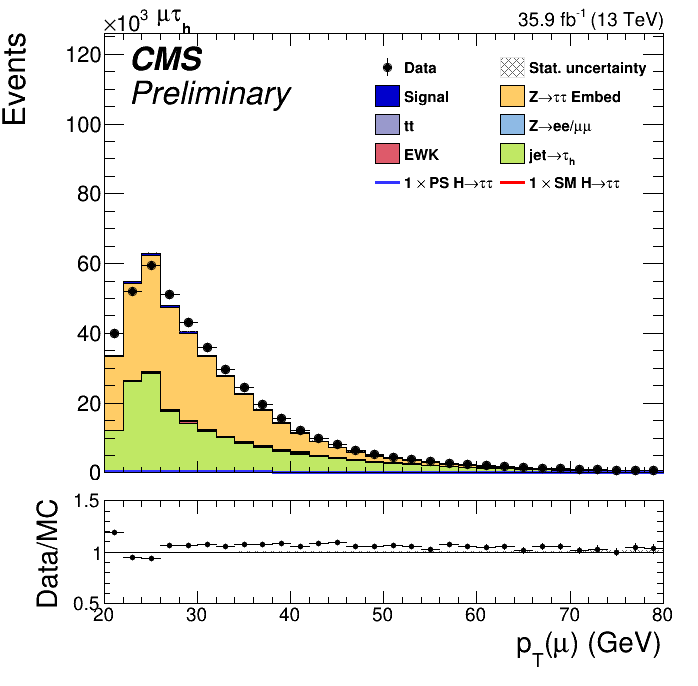
\includegraphics[width=\linewidth]{Chapitre7/Images/CtrlPlots/2016/MuonpT.png} 
    \caption{$p^{\mu}_T$, 2016.} 
    \vspace{0.5ex}
  \end{subfigure}%% 
  \begin{subfigure}[b]{0.33\linewidth}
    \centering
    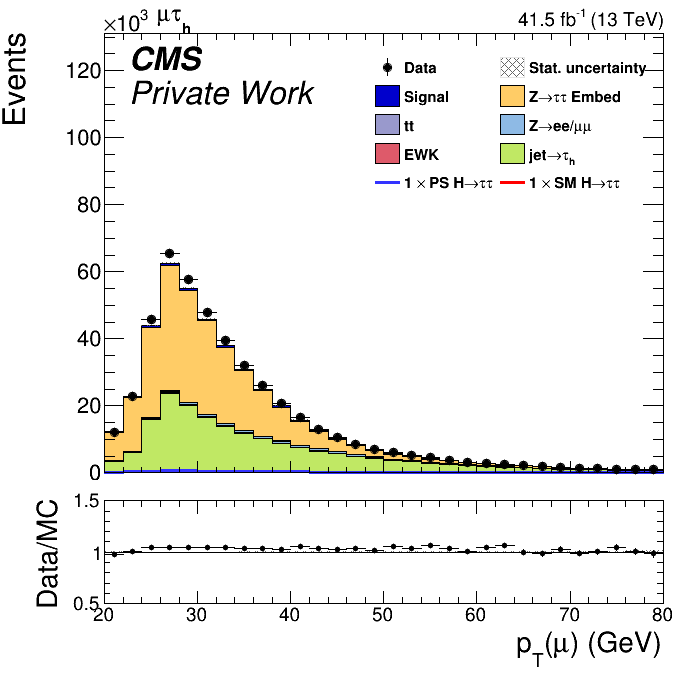
\includegraphics[width=\linewidth]{Chapitre7/Images/CtrlPlots/2017/MuonpT.png} 
    \caption{$p^{\mu}_T$, 2017.} 
    \vspace{0.5ex}
  \end{subfigure} 
    \begin{subfigure}[b]{0.33\linewidth}
    \centering
    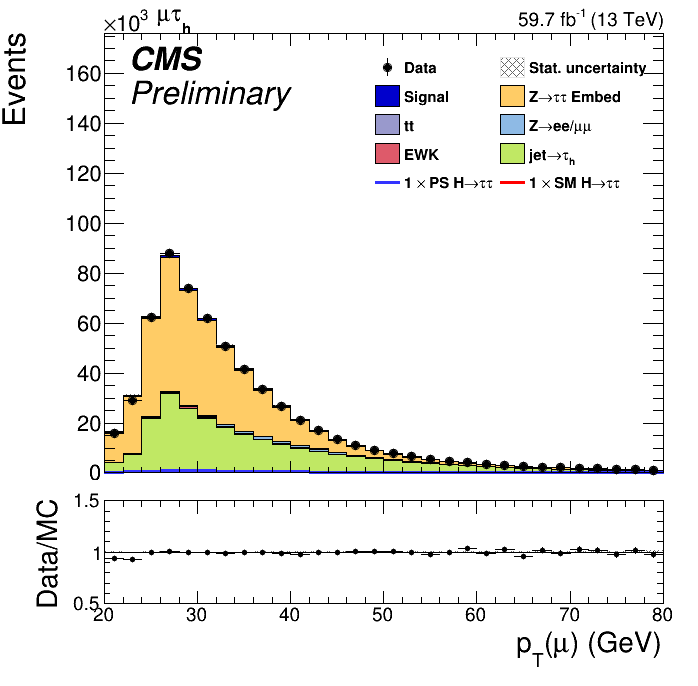
\includegraphics[width=\linewidth]{Chapitre7/Images/CtrlPlots/2018/MuonpT.png} 
    \caption{$p^{\mu}_T$, 2018.} 
    \vspace{0.5ex}
  \end{subfigure} 

    \begin{subfigure}[b]{0.33\linewidth}
    \centering
    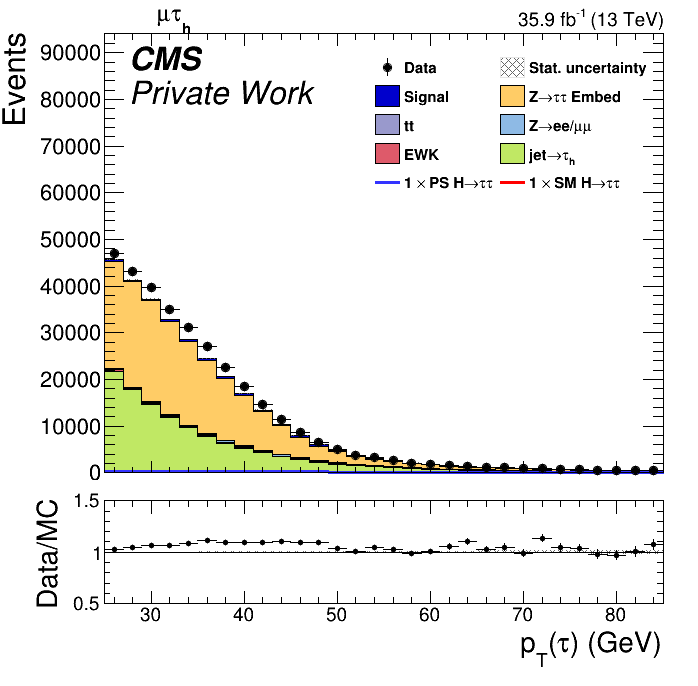
\includegraphics[width=\linewidth]{Chapitre7/Images/CtrlPlots/2016/TaupT.png} 
    \caption{$p^{\tau_h}_T$, 2016.} 
    \vspace{0.5ex}
  \end{subfigure}%% 
  \begin{subfigure}[b]{0.33\linewidth}
    \centering
    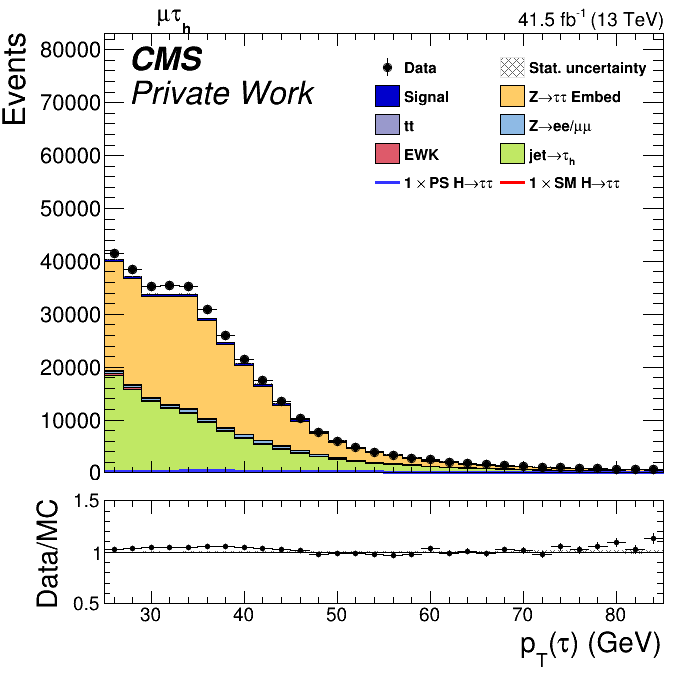
\includegraphics[width=\linewidth]{Chapitre7/Images/CtrlPlots/2017/TaupT.png} 
    \caption{$p^{\tau_h}_T$, 2017.} 
    \vspace{0.5ex}
  \end{subfigure} 
    \begin{subfigure}[b]{0.33\linewidth}
    \centering
    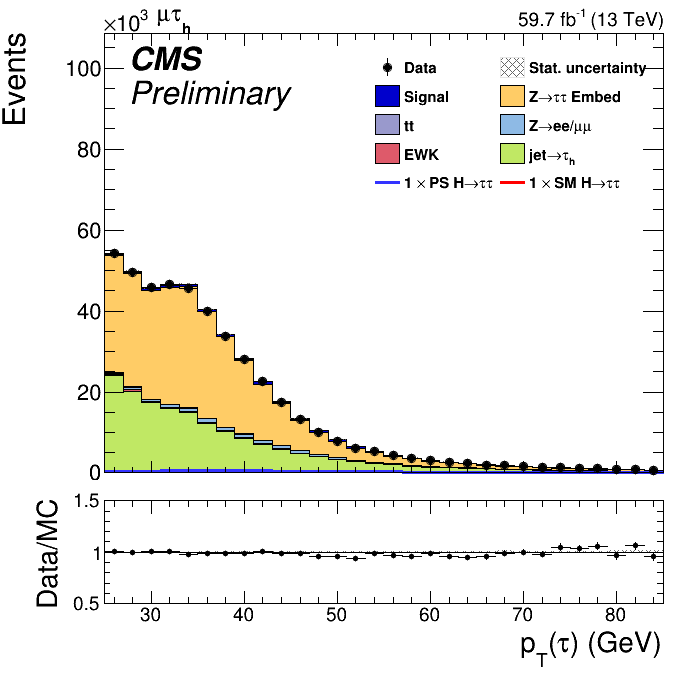
\includegraphics[width=\linewidth]{Chapitre7/Images/CtrlPlots/2018/TaupT.png} 
    \caption{$p^{\tau_h}_T$, 2018.} 
    \vspace{0.5ex}
  \end{subfigure}
  
  \begin{subfigure}[b]{0.33\linewidth}
    \centering
    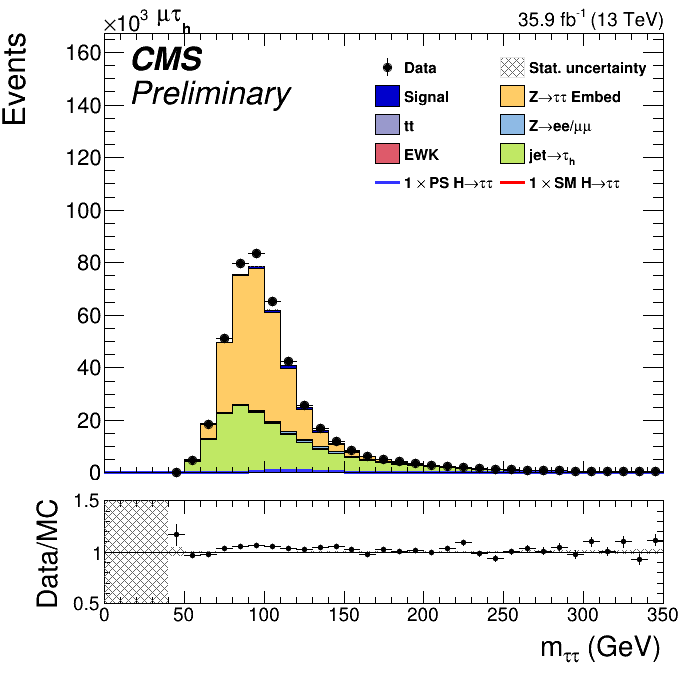
\includegraphics[width=\linewidth]{Chapitre7/Images/CtrlPlots/2016/fastMTTditauMass.png} 
    \caption{Fast MTT $m_{\tau\tau}$, 2016.} 
    \vspace{0.5ex}
  \end{subfigure}%% 
  \begin{subfigure}[b]{0.33\linewidth}
    \centering
    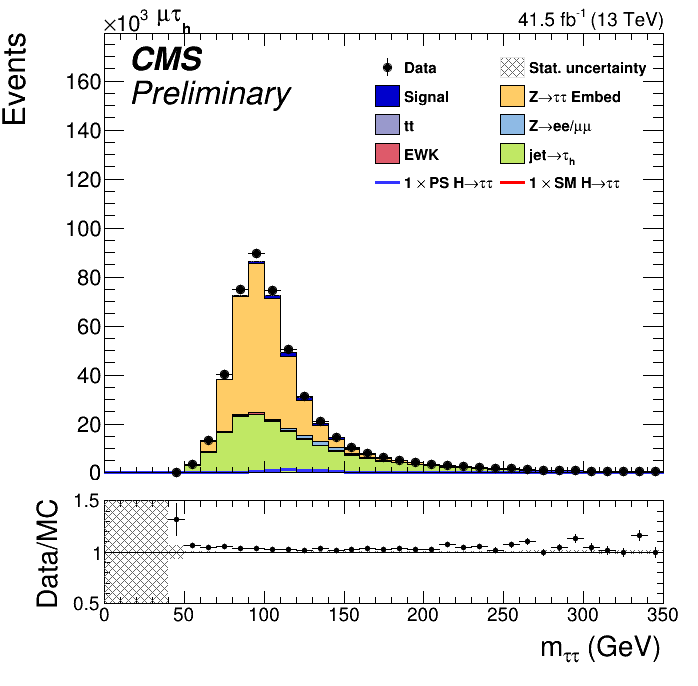
\includegraphics[width=\linewidth]{Chapitre7/Images/CtrlPlots/2017/fastMTTditauMass.png} 
    \caption{Fast MTT $m_{\tau\tau}$, 2017.} 
    \vspace{0.5ex}
  \end{subfigure} 
    \begin{subfigure}[b]{0.33\linewidth}
    \centering
    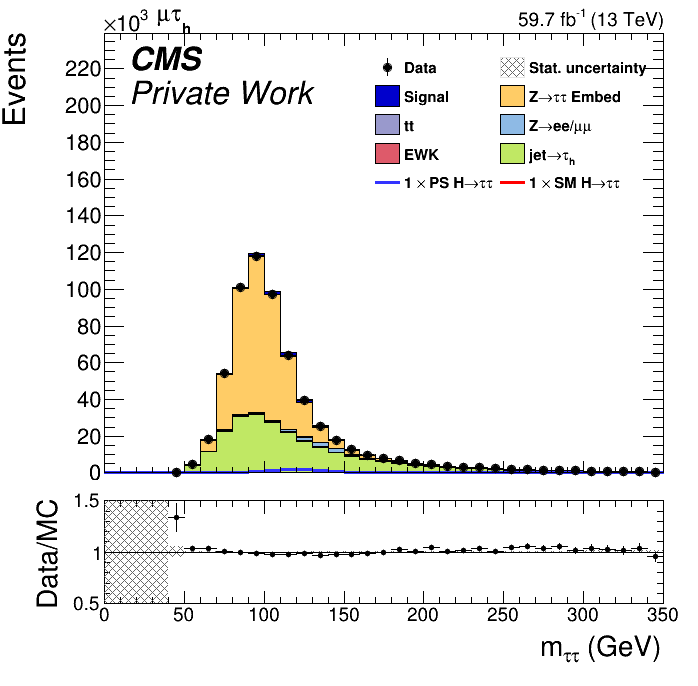
\includegraphics[width=\linewidth]{Chapitre7/Images/CtrlPlots/2018/fastMTTditauMass.png} 
    \caption{Fast MTT $m_{\tau\tau}$, 2018.} 
    \vspace{0.5ex}
  \end{subfigure} 

    \begin{subfigure}[b]{0.33\linewidth}
    \centering
    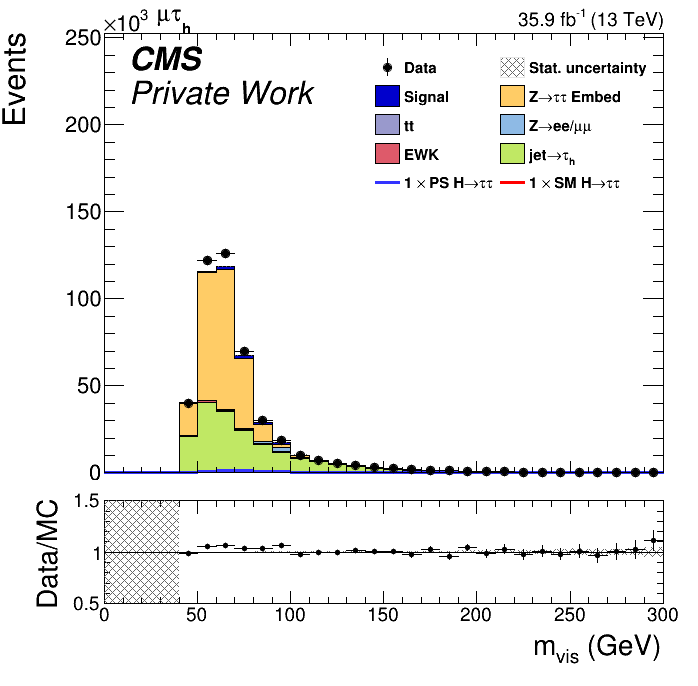
\includegraphics[width=\linewidth]{Chapitre7/Images/CtrlPlots/2016/VisibleMass.png} 
    \caption{$m_{\tau\tau}^{vis}$, 2016.} 
    \vspace{0.5ex}
  \end{subfigure}%% 
  \begin{subfigure}[b]{0.33\linewidth}
    \centering
    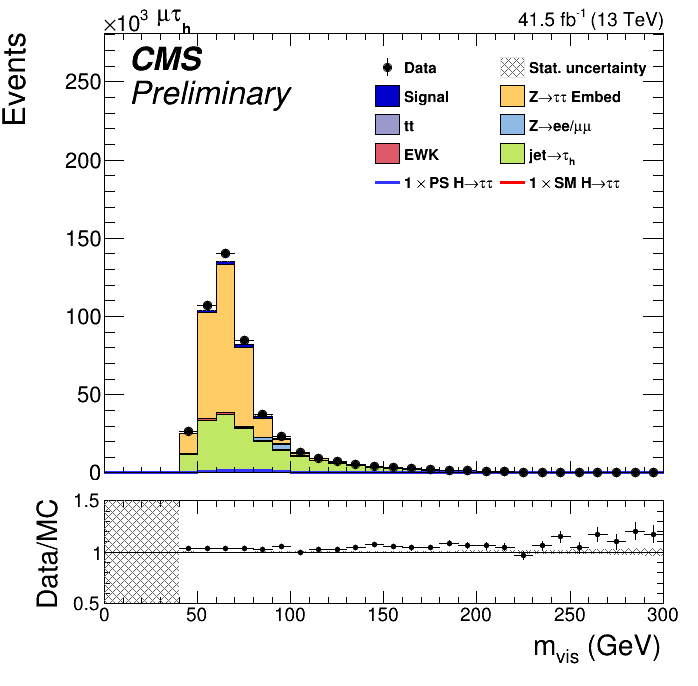
\includegraphics[width=\linewidth]{Chapitre7/Images/CtrlPlots/2017/VisibleMass.png} 
    \caption{$m_{\tau\tau}^{vis}$, 2017.} 
    \vspace{0.5ex}
  \end{subfigure} 
    \begin{subfigure}[b]{0.33\linewidth}
    \centering
    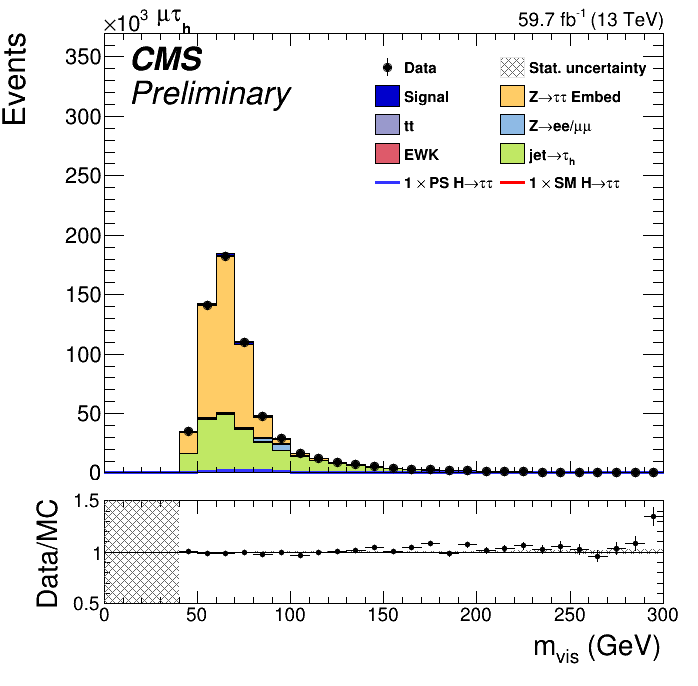
\includegraphics[width=\linewidth]{Chapitre7/Images/CtrlPlots/2018/VisibleMass.png} 
    \caption{$m_{\tau\tau}^{vis}$, 2018.} 
    \vspace{0.5ex}
  \end{subfigure} 
  \caption{}
  \label{page1}
\end{figure}

%page2
\begin{figure}
  \begin{subfigure}[b]{0.33\linewidth}
    \centering
    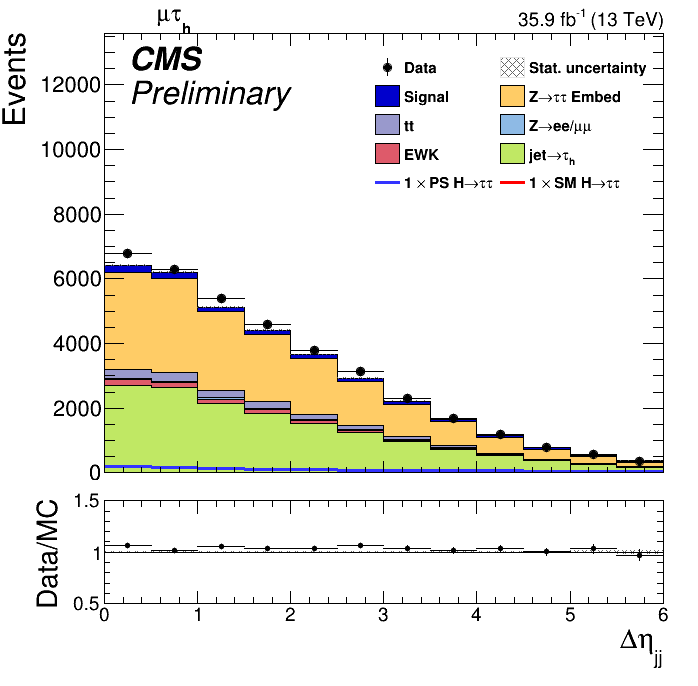
\includegraphics[width=\linewidth]{Chapitre7/Images/CtrlPlots/2016/DijetDeltaEta.png} 
    \caption{$|\Delta\eta|(jj)$, 2016.} 
    \vspace{0.5ex}
  \end{subfigure}%% 
  \begin{subfigure}[b]{0.33\linewidth}
    \centering
    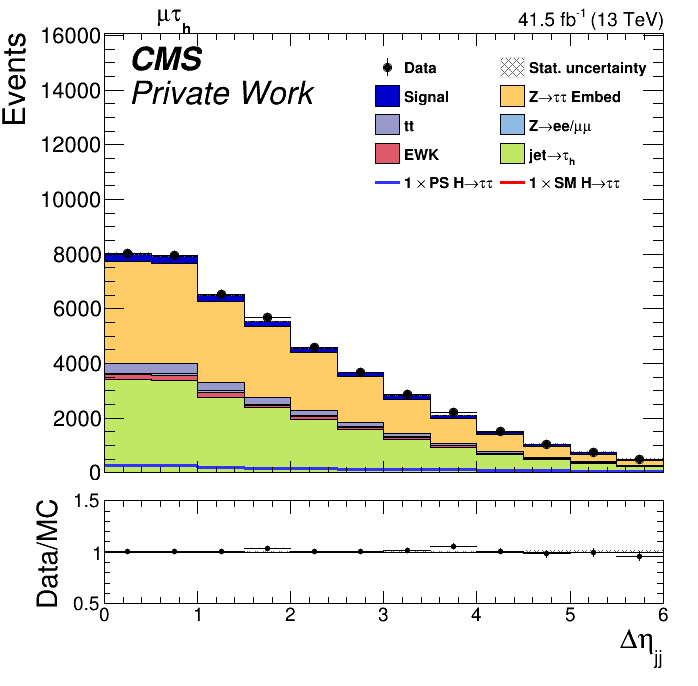
\includegraphics[width=\linewidth]{Chapitre7/Images/CtrlPlots/2017/DijetDeltaEta.png} 
    \caption{$|\Delta\eta|(jj)$, 2017.} 
    \vspace{0.5ex}
  \end{subfigure} 
    \begin{subfigure}[b]{0.33\linewidth}
    \centering
    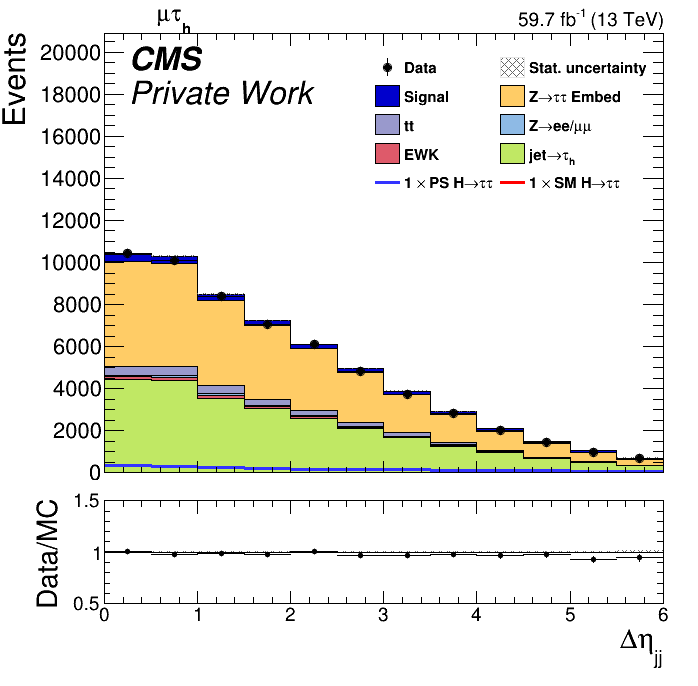
\includegraphics[width=\linewidth]{Chapitre7/Images/CtrlPlots/2018/DijetDeltaEta.png} 
    \caption{$|\Delta\eta|(jj)$, 2018.} 
    \vspace{0.5ex}
  \end{subfigure} 

  \begin{subfigure}[b]{0.33\linewidth}
    \centering
    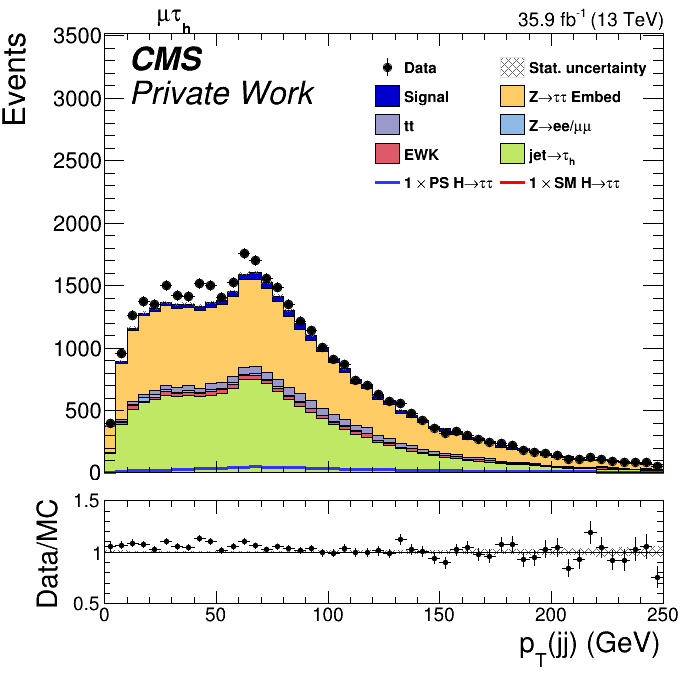
\includegraphics[width=\linewidth]{Chapitre7/Images/CtrlPlots/2016/DijetpT.png} 
    \caption{$p_T(jj)$, 2016.} 
    \vspace{0.5ex}
  \end{subfigure}%% 
  \begin{subfigure}[b]{0.33\linewidth}
    \centering
    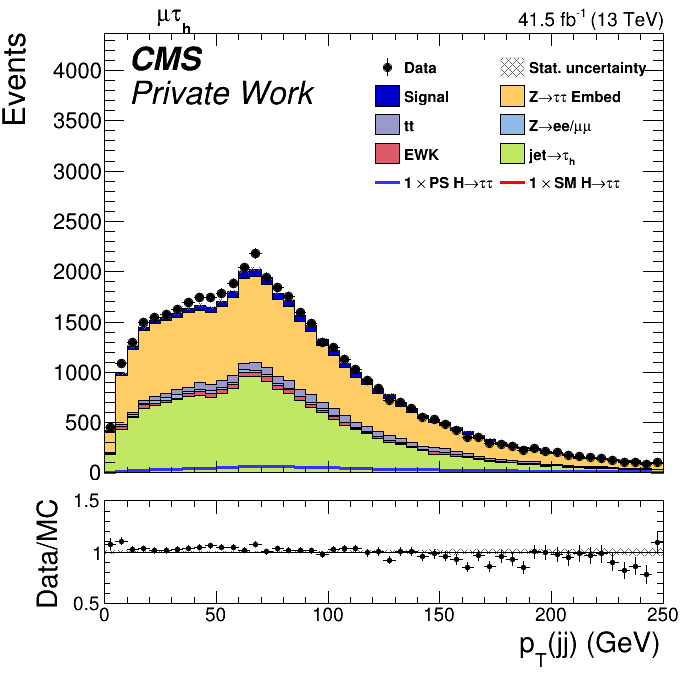
\includegraphics[width=\linewidth]{Chapitre7/Images/CtrlPlots/2017/DijetpT.png} 
    \caption{$p_T(jj)$, 2017.} 
    \vspace{0.5ex}
  \end{subfigure} 
    \begin{subfigure}[b]{0.33\linewidth}
    \centering
    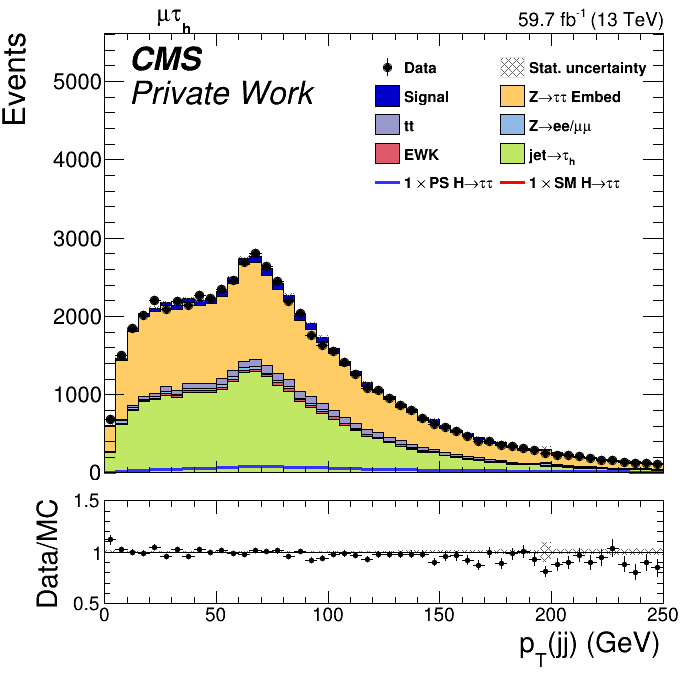
\includegraphics[width=\linewidth]{Chapitre7/Images/CtrlPlots/2018/DijetpT.png} 
    \caption{$p_T(jj)$, 2018.} 
    \vspace{0.5ex}
  \end{subfigure} 

  \begin{subfigure}[b]{0.33\linewidth}
    \centering
    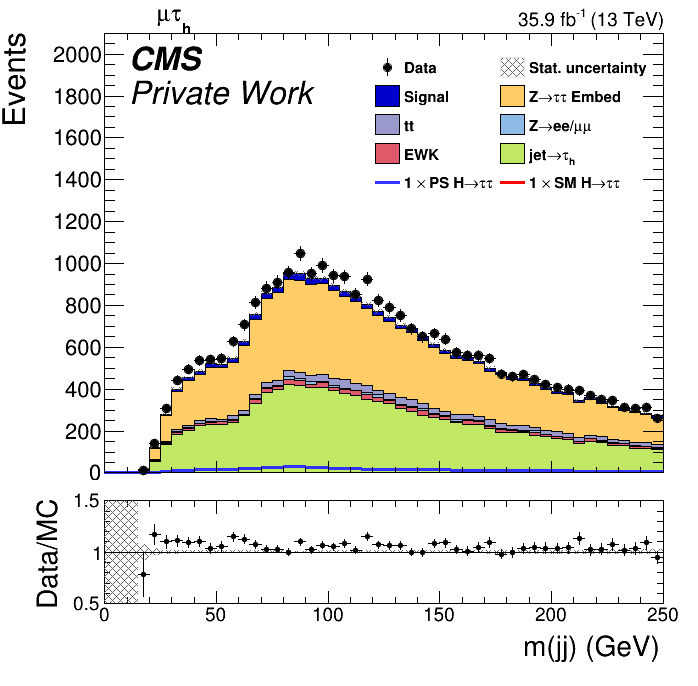
\includegraphics[width=\linewidth]{Chapitre7/Images/CtrlPlots/2016/DijetMass.png} 
    \caption{$m(jj)$, 2016.} 
    \vspace{0.5ex}
  \end{subfigure}%% 
  \begin{subfigure}[b]{0.33\linewidth}
    \centering
    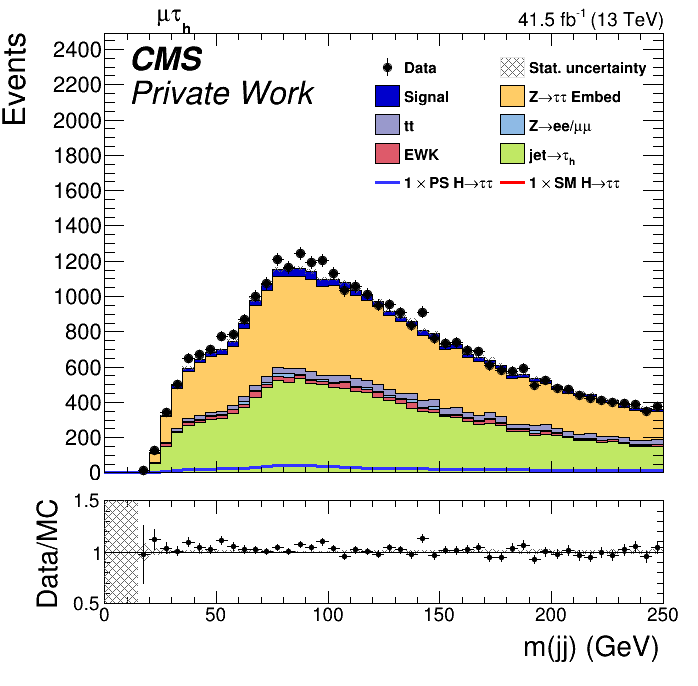
\includegraphics[width=\linewidth]{Chapitre7/Images/CtrlPlots/2017/DijetMass.png} 
    \caption{$m(jj)$, 2017.} 
    \vspace{0.5ex}
  \end{subfigure} 
    \begin{subfigure}[b]{0.33\linewidth}
    \centering
    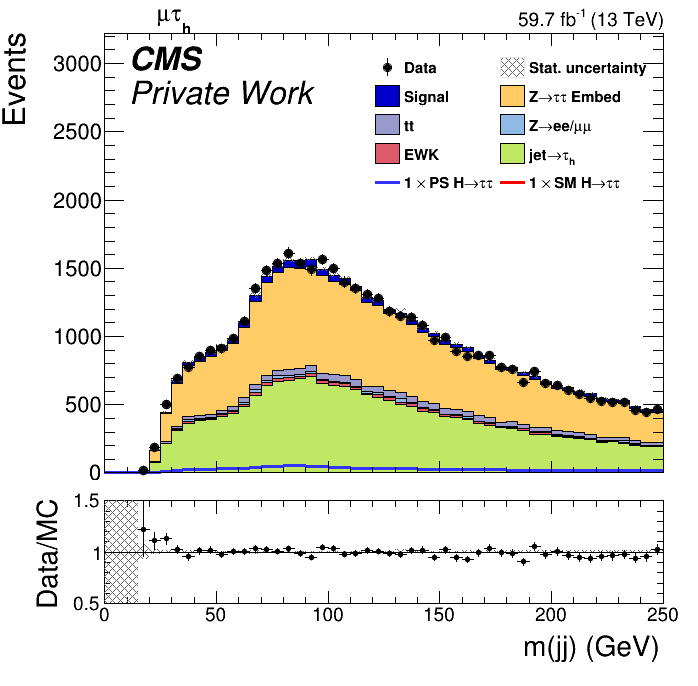
\includegraphics[width=\linewidth]{Chapitre7/Images/CtrlPlots/2018/DijetMass.png} 
    \caption{$m(jj)$, 2018.} 
    \vspace{0.5ex}
  \end{subfigure} 

    \begin{subfigure}[b]{0.33\linewidth}
    \centering
    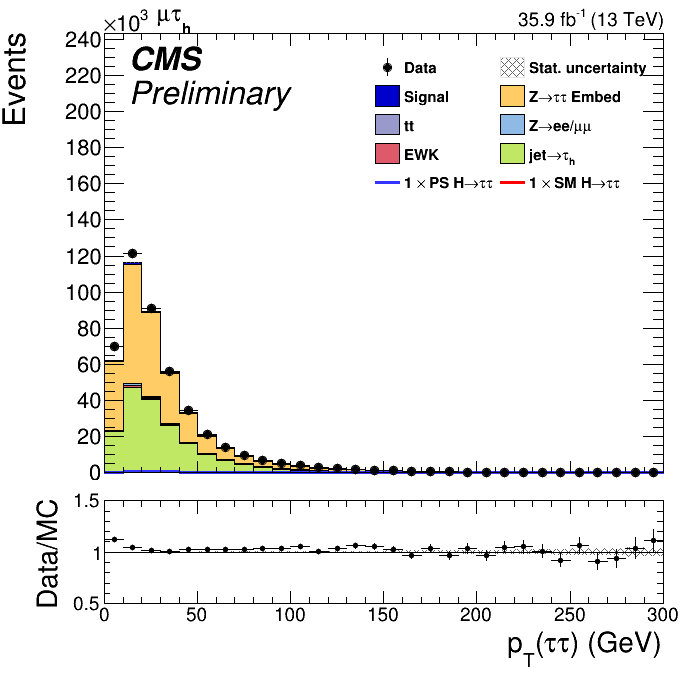
\includegraphics[width=\linewidth]{Chapitre7/Images/CtrlPlots/2016/DitaupT.png} 
    \caption{$p^{\tau\tau}_T$, 2016.} 
    \vspace{0.5ex}
  \end{subfigure}%% 
  \begin{subfigure}[b]{0.33\linewidth}
    \centering
    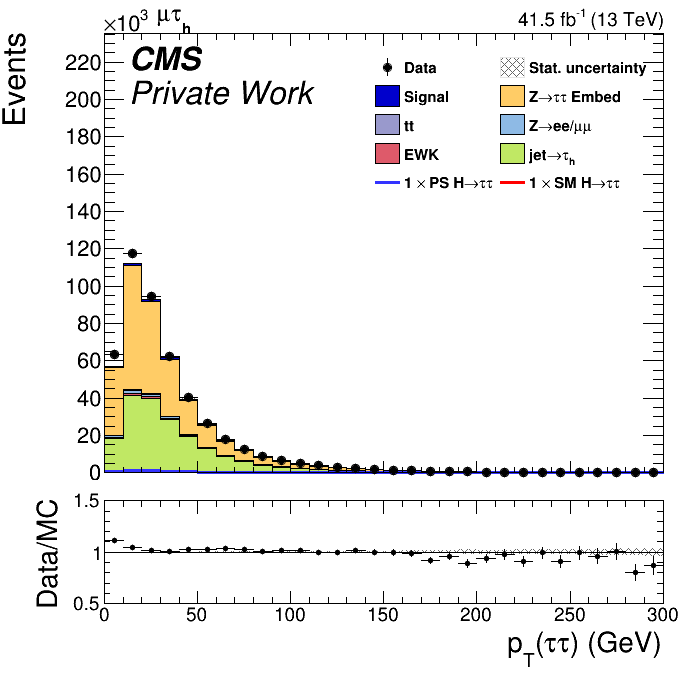
\includegraphics[width=\linewidth]{Chapitre7/Images/CtrlPlots/2017/DitaupT.png} 
    \caption{$p^{\tau\tau}_T$, 2017.} 
    \vspace{0.5ex}
  \end{subfigure} 
    \begin{subfigure}[b]{0.33\linewidth}
    \centering
    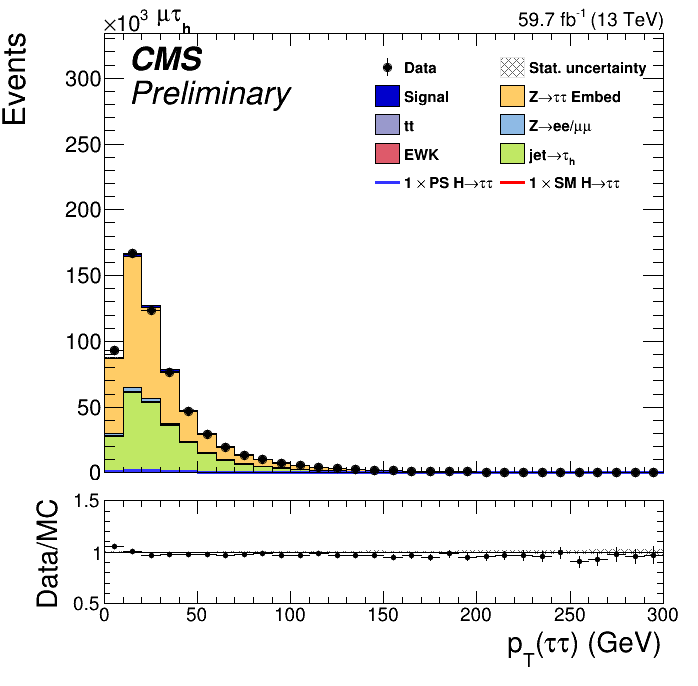
\includegraphics[width=\linewidth]{Chapitre7/Images/CtrlPlots/2018/DitaupT.png} 
    \caption{$p^{\tau\tau}_T$, 2018.} 
    \vspace{0.5ex}
  \end{subfigure} 
  \caption{}
  \label{page2}
\end{figure}

%page3
\begin{figure}
  \begin{subfigure}[b]{0.33\linewidth}
    \centering
    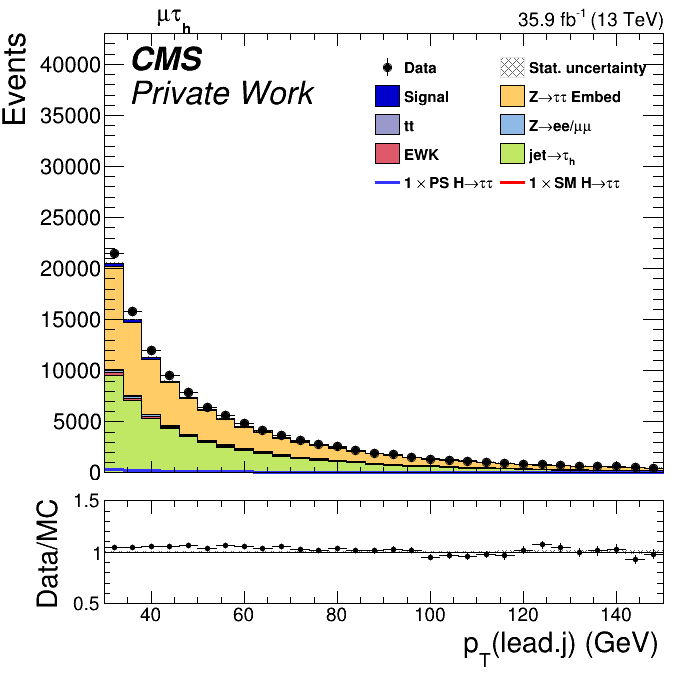
\includegraphics[width=\linewidth]{Chapitre7/Images/CtrlPlots/2016/LeadingJetpT.png} 
    \caption{Leading jet $p_T$, 2016.} 
    \vspace{0.5ex}
  \end{subfigure}%% 
  \begin{subfigure}[b]{0.33\linewidth}
    \centering
    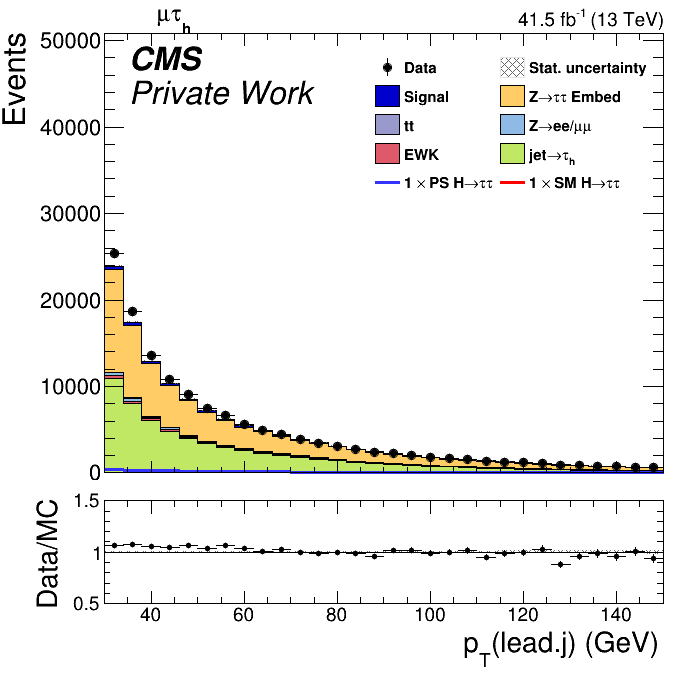
\includegraphics[width=\linewidth]{Chapitre7/Images/CtrlPlots/2017/LeadingJetpT.png} 
    \caption{Leading jet $p_T$, 2017.} 
    \vspace{0.5ex}
  \end{subfigure} 
    \begin{subfigure}[b]{0.33\linewidth}
    \centering
    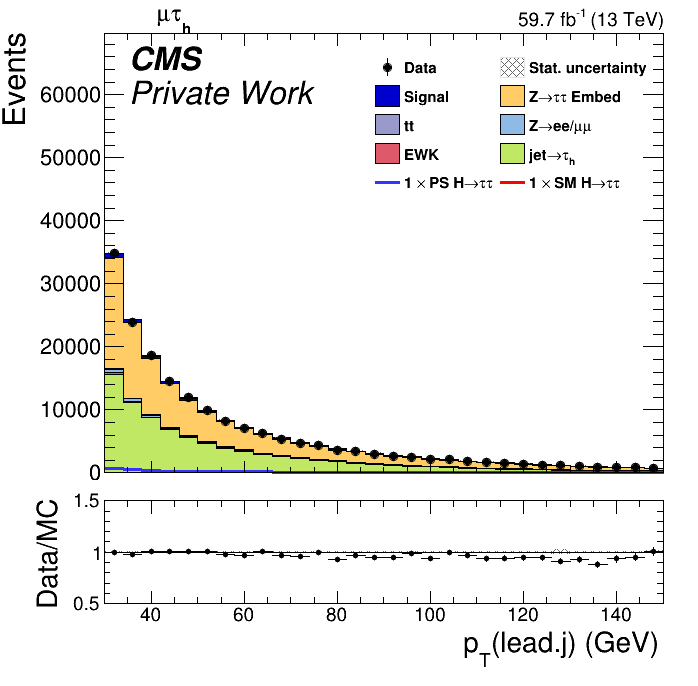
\includegraphics[width=\linewidth]{Chapitre7/Images/CtrlPlots/2018/LeadingJetpT.png} 
    \caption{Leading jet $p_T$, 2018.} 
    \vspace{0.5ex}
  \end{subfigure} 

    \begin{subfigure}[b]{0.33\linewidth}
    \centering
    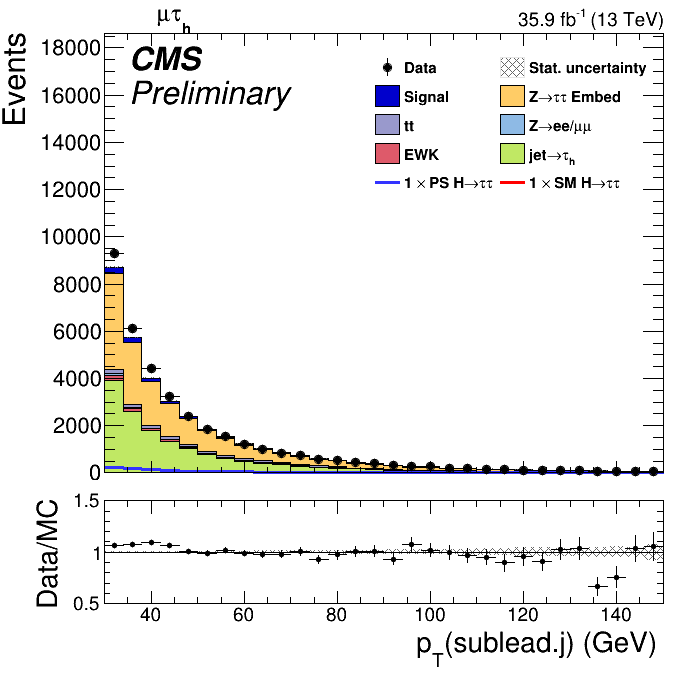
\includegraphics[width=\linewidth]{Chapitre7/Images/CtrlPlots/2016/SubleadingJetpT.png} 
    \caption{Subleading jet $p_T$, 2016.} 
    \vspace{0.5ex}
  \end{subfigure}%% 
  \begin{subfigure}[b]{0.33\linewidth}
    \centering
    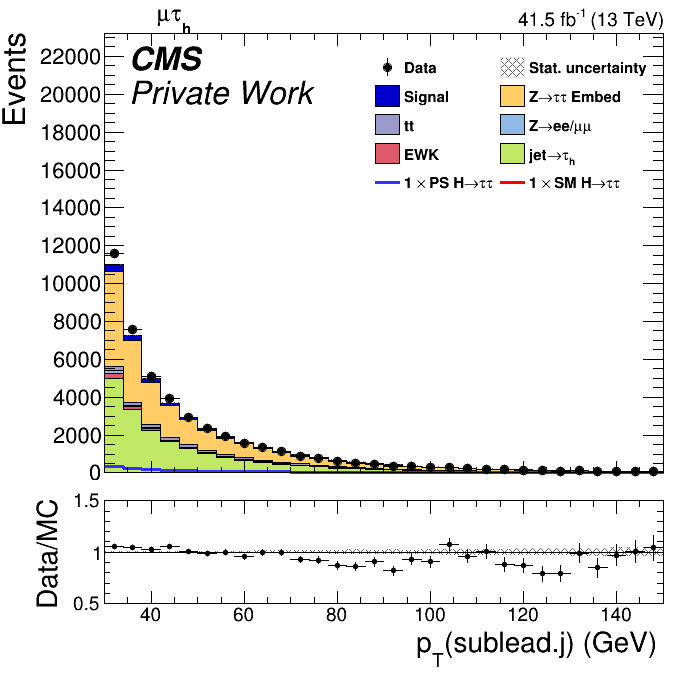
\includegraphics[width=\linewidth]{Chapitre7/Images/CtrlPlots/2017/SubleadingJetpT.png} 
    \caption{Subleading jet $p_T$, 2017.} 
    \vspace{0.5ex}
  \end{subfigure} 
    \begin{subfigure}[b]{0.33\linewidth}
    \centering
    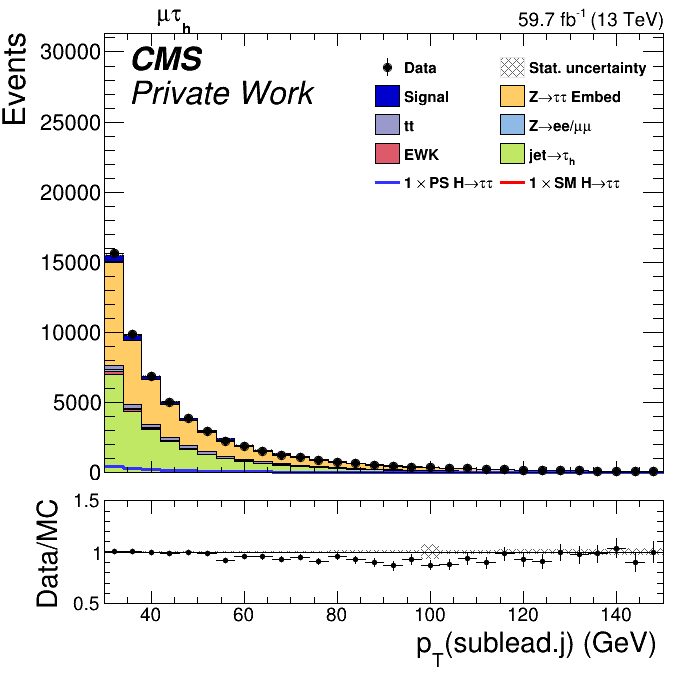
\includegraphics[width=\linewidth]{Chapitre7/Images/CtrlPlots/2018/SubleadingJetpT.png} 
    \caption{Subleading jet $p_T$, 2018.} 
    \vspace{0.5ex}
  \end{subfigure}
  
  \begin{subfigure}[b]{0.33\linewidth}
    \centering
    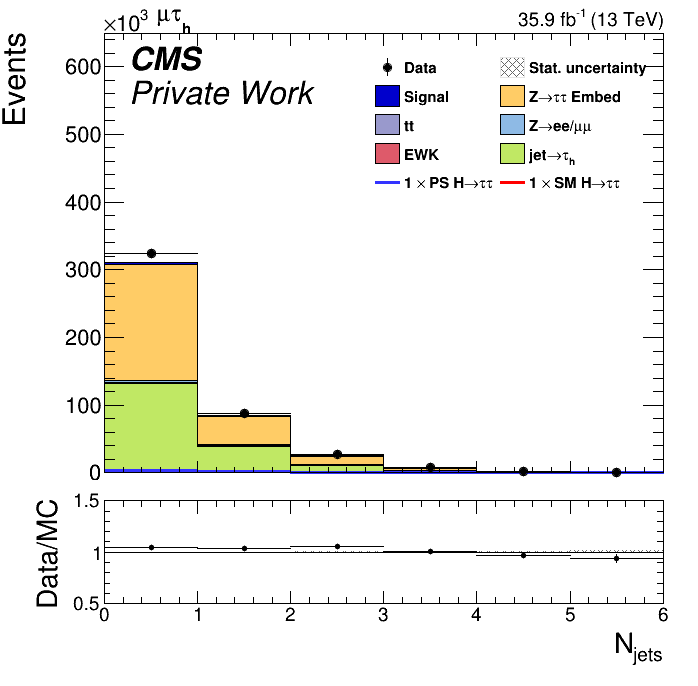
\includegraphics[width=\linewidth]{Chapitre7/Images/CtrlPlots/2016/Njets.png} 
    \caption{$N$ jets, 2016.} 
    \vspace{0.5ex}
  \end{subfigure}%% 
  \begin{subfigure}[b]{0.33\linewidth}
    \centering
    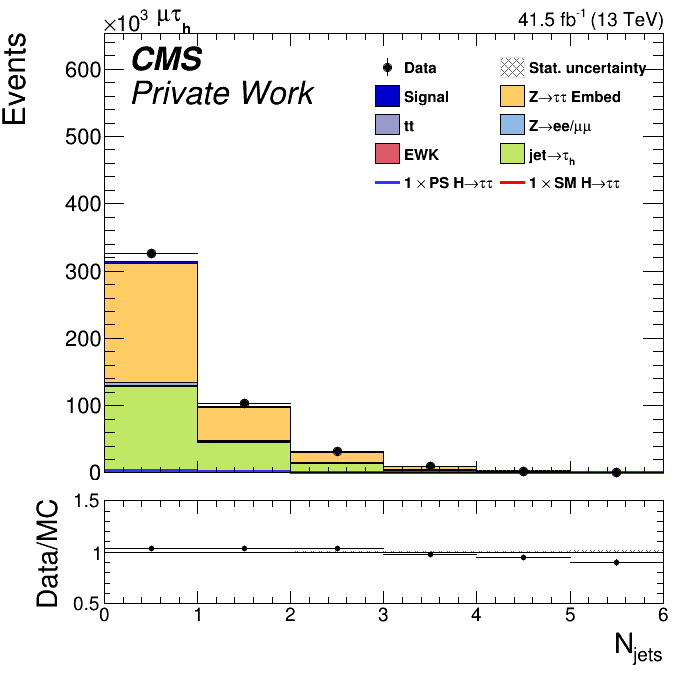
\includegraphics[width=\linewidth]{Chapitre7/Images/CtrlPlots/2017/Njets.png} 
    \caption{$N$ jets, 2017.} 
    \vspace{0.5ex}
  \end{subfigure} 
    \begin{subfigure}[b]{0.33\linewidth}
    \centering
    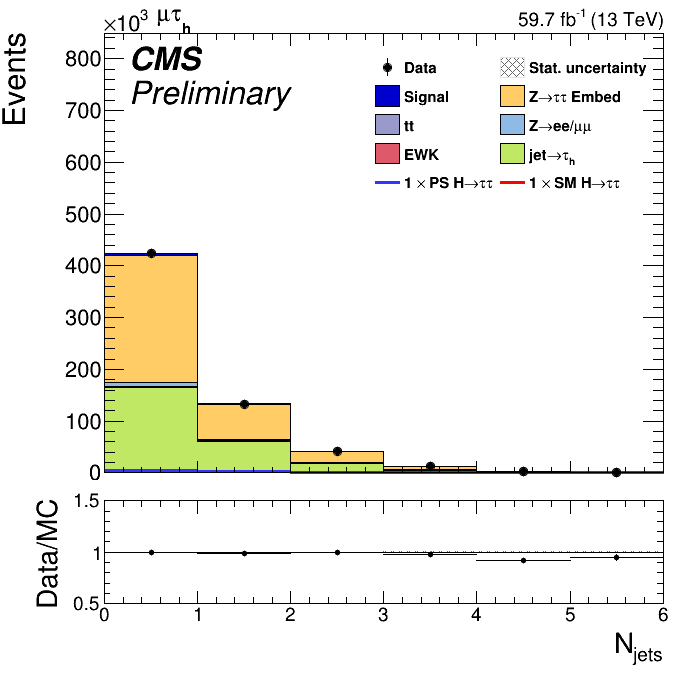
\includegraphics[width=\linewidth]{Chapitre7/Images/CtrlPlots/2018/Njets.png} 
    \caption{$N$ jets, 2018.} 
    \vspace{0.5ex}
  \end{subfigure} 

    \begin{subfigure}[b]{0.33\linewidth}
    \centering
    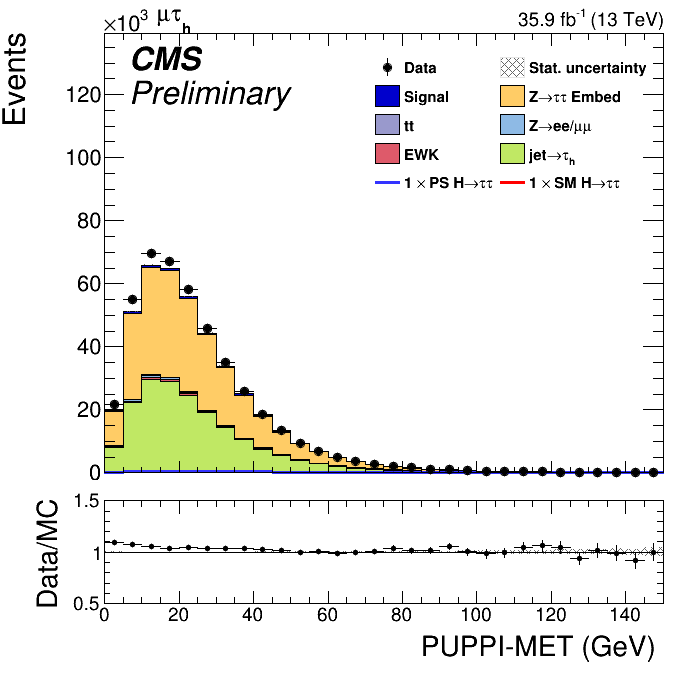
\includegraphics[width=\linewidth]{Chapitre7/Images/CtrlPlots/2016/PUPPImet.png} 
    \caption{$p^{mis}_T$, 2016.} 
    \vspace{0.5ex}
  \end{subfigure}%% 
  \begin{subfigure}[b]{0.33\linewidth}
    \centering
    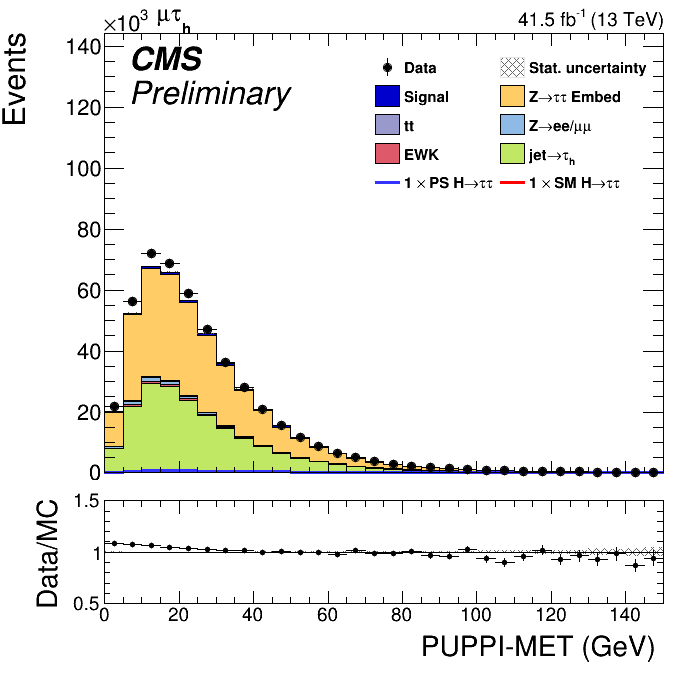
\includegraphics[width=\linewidth]{Chapitre7/Images/CtrlPlots/2017/PUPPImet.png} 
    \caption{$p^{mis}_T$, 2017.} 
    \vspace{0.5ex}
  \end{subfigure} 
    \begin{subfigure}[b]{0.33\linewidth}
    \centering
    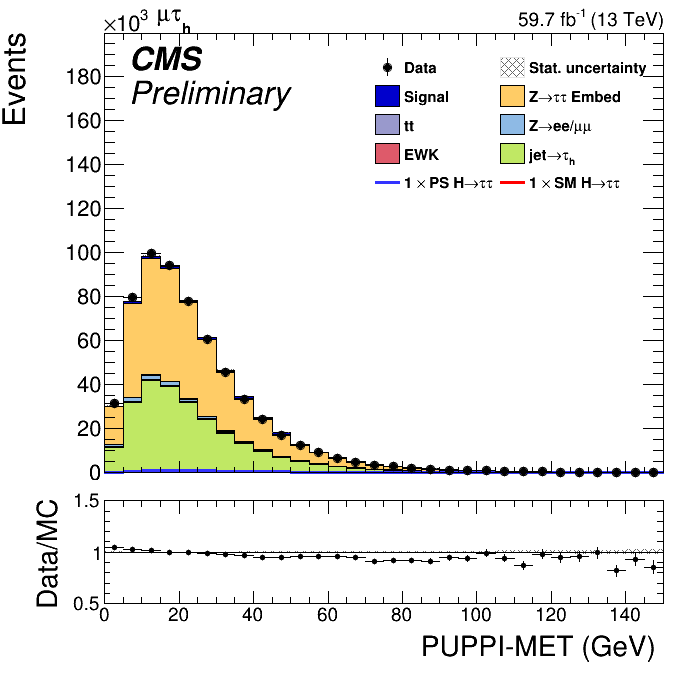
\includegraphics[width=\linewidth]{Chapitre7/Images/CtrlPlots/2018/PUPPImet.png} 
    \caption{$p^{mis}_T$, 2018.} 
    \vspace{0.5ex}
  \end{subfigure} 
  \caption{}
  \label{page3}
\end{figure}

\begin{figure}
    \begin{subfigure}[b]{0.33\linewidth}
    \centering
    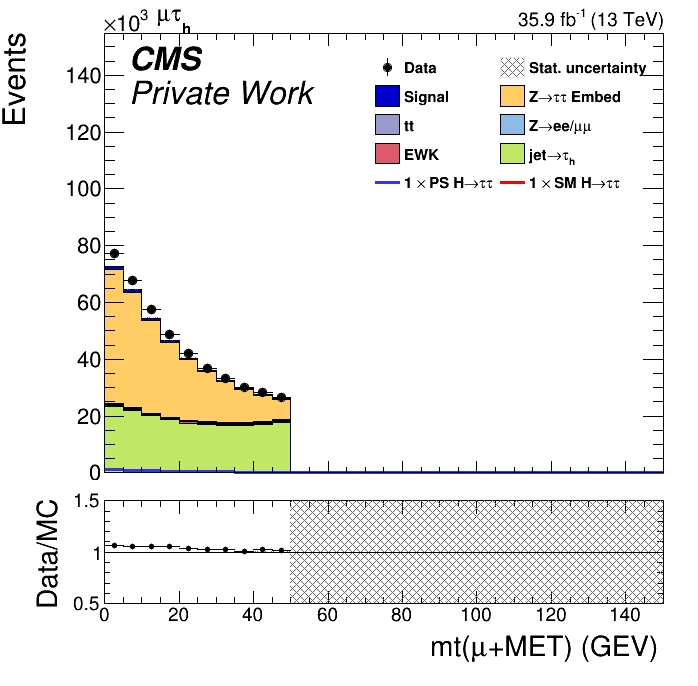
\includegraphics[width=\linewidth]{Chapitre7/Images/CtrlPlots/2016/MuMETmt.png} 
    \caption{$m^{\mu+MET}_T$, 2016.} 
    \vspace{0.5ex}
  \end{subfigure}%% 
  \begin{subfigure}[b]{0.33\linewidth}
    \centering
    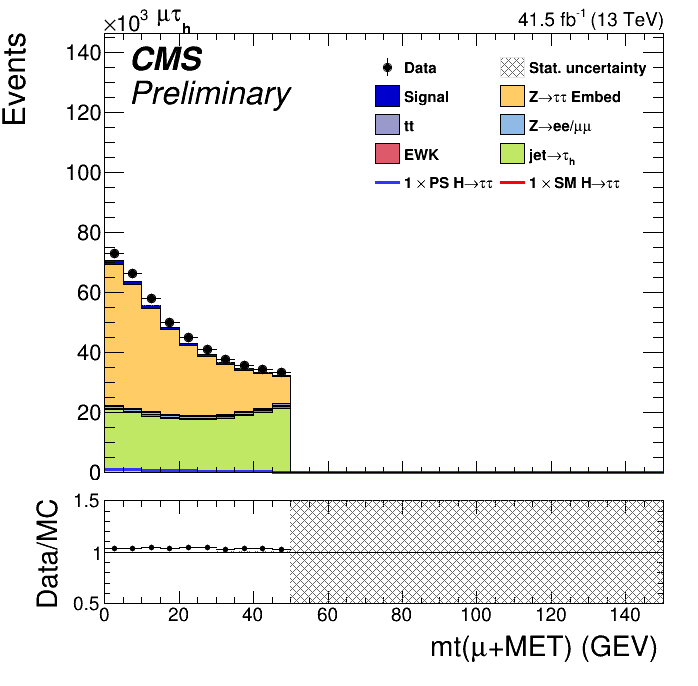
\includegraphics[width=\linewidth]{Chapitre7/Images/CtrlPlots/2017/MuMETmt.png} 
    \caption{$m^{\mu+MET}_T$, 2017.} 
    \vspace{0.5ex}
  \end{subfigure} 
    \begin{subfigure}[b]{0.33\linewidth}
    \centering
    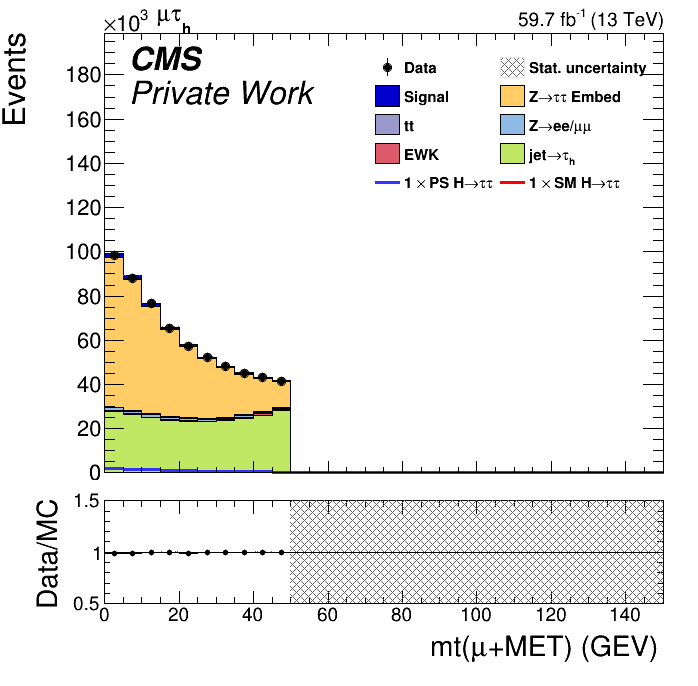
\includegraphics[width=\linewidth]{Chapitre7/Images/CtrlPlots/2018/MuMETmt.png} 
    \caption{$m^{\mu+MET}_T$, 2018.} 
    \vspace{0.5ex}
  \end{subfigure} 
  \caption{}
  \label{page4}
\end{figure}

Distribution du score de sortie du BDT dans la catégorie Jet Fakes (a), $Z\rightarrow\tau\tau$ Embed (b) et Higgs (c) pour les données de 2018. Les données sont masquées dans la troisième catégorie dans laquelle le signal est attendu.

\begin{figure}[!ht]
    \begin{subfigure}[b]{0.33\linewidth}
    \centering
    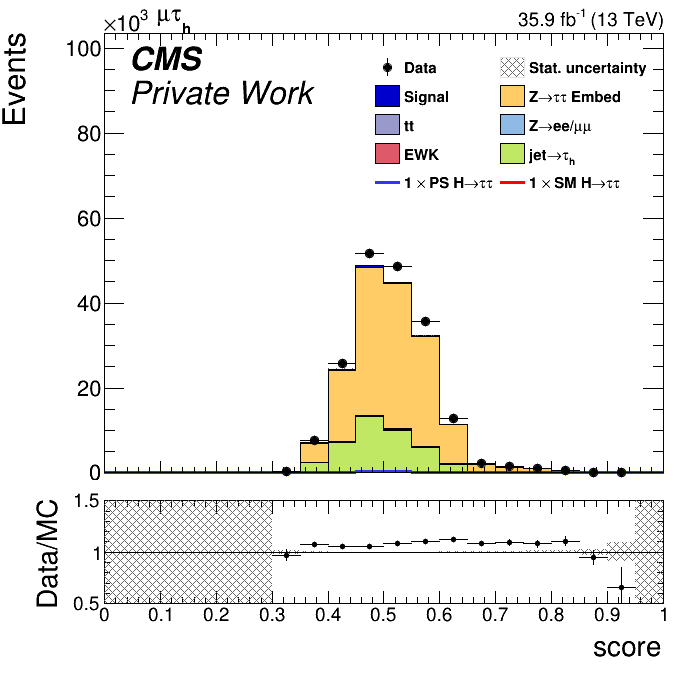
\includegraphics[width=\linewidth]{Chapitre7/Images/CtrlPlots/2016/BDTscoreZTT.png} 
    \caption{$Z\to\tau\tau$, 2016.} 
    \vspace{0.5cm}
  \end{subfigure}%% 
  \begin{subfigure}[b]{0.33\linewidth}
    \centering
    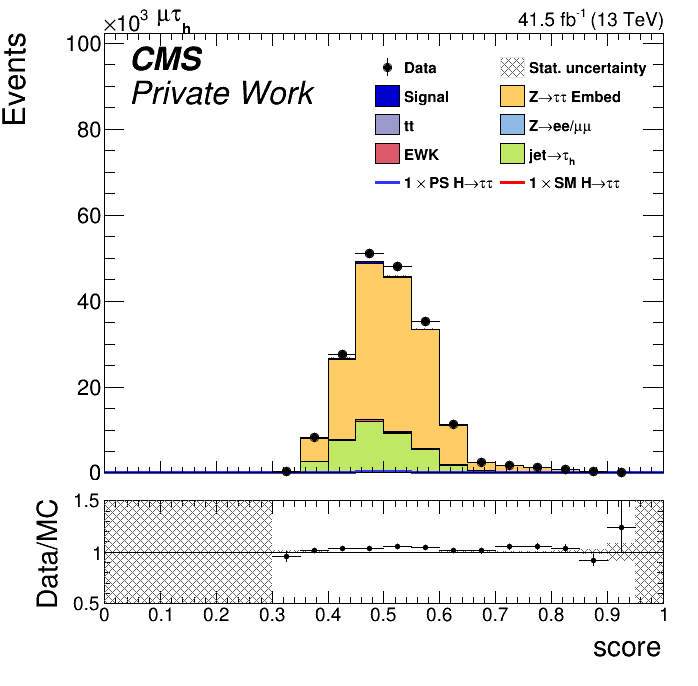
\includegraphics[width=\linewidth]{Chapitre7/Images/CtrlPlots/2017/BDTscoreZTT.png} 
    \caption{$Z\to\tau\tau$, 2017.} 
    \vspace{0.5cm}
  \end{subfigure} 
    \begin{subfigure}[b]{0.33\linewidth}
    \centering
    \includegraphics[width=\linewidth]{Chapitre7/Images/CtrlPlots/2018/BDTscoreZTT.png} 
    \caption{$Z\to\tau\tau$, 2018.} 
    \vspace{0.5cm}
  \end{subfigure} 
  %%
  \begin{subfigure}[b]{0.33\linewidth}
    \centering
    \includegraphics[width=\linewidth]{Chapitre7/Images/CtrlPlots/2016/BDTscoreJetFakes.png} 
    \caption{JetFakes, 2016.} 
    \vspace{0.5cm}
  \end{subfigure}%% 
  \begin{subfigure}[b]{0.33\linewidth}
    \centering
    \includegraphics[width=\linewidth]{Chapitre7/Images/CtrlPlots/2017/BDTscoreJetFakes.png} 
    \caption{JetFakes, 2017.} 
    \vspace{0.5cm}
  \end{subfigure} 
    \begin{subfigure}[b]{0.33\linewidth}
    \centering
    \includegraphics[width=\linewidth]{Chapitre7/Images/CtrlPlots/2018/BDTscoreJetFakes.png} 
    \caption{JetFakes, 2018.} 
    \vspace{0.5cm}
  \end{subfigure} 
  %%
  \begin{subfigure}[b]{0.33\linewidth}
    \centering
    \includegraphics[width=\linewidth]{Chapitre7/Images/CtrlPlots/2016/BDTscoreHiggs.png} 
    \caption{Higgs, 2016.} 
    \vspace{0.5ex}
  \end{subfigure}%% 
  \begin{subfigure}[b]{0.33\linewidth}
    \centering
    \includegraphics[width=\linewidth]{Chapitre7/Images/CtrlPlots/2017/BDTscoreHiggs.png} 
    \caption{Higgs, 2017.} 
    \vspace{0.5ex}
  \end{subfigure} 
    \begin{subfigure}[b]{0.33\linewidth}
    \centering
    \includegraphics[width=\linewidth]{Chapitre7/Images/CtrlPlots/2018/BDTscoreHiggs.png} 
    \caption{Higgs, 2018.} 
    \vspace{0.5ex}
  \end{subfigure} 
  \caption{Distribution du score de sortie du BDT dans la catégorie $Z\to\tau\tau$ (haut), \textit{jetFakes} (milieu) et Higgs (bas) pour les données de 2016, 0271 et 2018. Les données sont masquées dans la troisième catégorie dans laquelle le signal est attendu.}
  \label{BDTscores}
\end{figure}

\begin{figure}
    \begin{subfigure}[b]{0.5\linewidth}
        \centering
        \includegraphics[scale=0.28]{Chapitre7/Images/CtrlPlots/2018/BDTscoreJetFakes.png} 
        \caption{} 
        \vspace{0.5ex}
    \end{subfigure}
    \begin{subfigure}[b]{0.5\linewidth}
        \centering
        \includegraphics[scale=0.28]{Chapitre7/Images/CtrlPlots/2018/BDTscoreZTT.png} 
        \caption{} 
        \vspace{0.5ex}
    \end{subfigure}
        \begin{subfigure}[b]{\linewidth}
        \centering
        \includegraphics[scale=0.28]{Chapitre7/Images/CtrlPlots/2018/BDTscoreHiggs.png} 
        \caption{} 
        \vspace{0.5ex}
    \end{subfigure}
    \caption{Distribution du score de sortie du BDT dans la catégorie Jet Fakes (a), $Z\rightarrow\tau\tau$ Embed (b) et Higgs (c) pour les données de 2018. Les données sont masquées dans la troisième catégorie dans laquelle le signal est attendu.}
    \label{BDTscores}
\end{figure}

\section{Extraction de $\alpha^{H\tau\tau}$}
\label{extract}

La classification des évènements présentées dans la section \ref{BDTclassifier} permet d'extraire une mesure du paramètre $\alpha^{H\tau\tau}$ dans les données par le maximum de vraisemblance. Un ajustement simultané dans chaque catégories de signal et de bruit de fond est réalisé grâce à l'outil Combine \cite{combine}. En plus de la mesure de $\alpha^{H\tau\tau}$, l'analyse vise également à mesurer l'intensité de signal $\mu$ de la désintégration $H\to\tau\tau$ dont l'expression en fonction des constantes de couplage $\kappa_{\tau}$ et $\tilde{\kappa}_{\tau}$ est donnée par 

\begin{equation}
  \mu=\kappa_{\tau}^2+\tilde{\kappa}_{\tau}^2.
\end{equation}

L'ajustement utilise en entrée une distribution dite \textit{unrolled} de l'observable $phi_{CP}$ dans le canal $a_1^{3pr}+\mu$ à partir des évènements de la catégorie de signal telle que présentée dans la figure \ref{unrolled}. Ces distributions sont obtenues à partir d'une distribution de $phi_{CP}$ répétée dans plusieurs intervalles de score. 

\subsection{Modèle d'ajustement}

La section \ref{CPsim} présente comment la distribution de $\phi_{CP}$ peut être paramétrisée pour une valeur quelconque de $\alpha^{H\tau\tau}$ à partir d'une combinaison linéaire des distributions pour $\alpha^{H\tau\tau}=0^\circ,45^\circ,90^\circ$. À partir de l'équation \ref{CPdiff}, le modèle de signal $S(\vv{\mu},\alpha^{H\tau\tau})$ utilisé pour l'extraction de l'angle de mélange $\alpha^{H\tau\tau}$ est défini par :

\begin{align}
    S(\vv{\mu},\alpha^{H\tau\tau}) & =\mathcal{L}\cdot\sum_{i}\mu_i\cdot\left(\frac{d\sigma}{d\phi_{CP}}\right)_i \nonumber \\[1em]
     & =\mathcal{L}\cdot\sum_{i}\mu_i\cdot \Biggl[\bigl(\cos^2\bigl(\alpha^{H\tau\tau}\bigr)-\sin\bigl(\alpha^{H\tau\tau}\bigr)\cos\bigl(\alpha^{H\tau\tau}\bigr)\bigr)\left(\frac{d\sigma^{CP-even}}{d\phi_{CP}}\right)_i \nonumber \\[1em] 
     & + \bigl(\sin^2\bigl(\alpha^{H\tau\tau}\bigr)-\sin\bigl(\alpha^{H\tau\tau}\bigr)\cos\bigl(\alpha^{H\tau\tau}\bigr)\bigr)\left(\frac{d\sigma^{CP-odd}}{d\phi_{CP}}\right)_i \nonumber \\[1em] 
     & + 2\sin\bigl(\alpha^{H\tau\tau}\bigr)\cos\bigl(\alpha^{H\tau\tau}\bigr)\left(\frac{d\sigma^{CP-mix}}{d\phi_{CP}}\right)_i\Biggr],
\end{align}

où $i$ désigne chaque mode de production du boson de Higgs, $\mathcal{L}$ désigne la luminosité intégrée et $\mu_i$ représente l'intensité de signal pour chaque mode de production. Cette dernière s'exprime sous la forme $$\mu_i=\mu_{ggH/V}\times\mathcal{B}^{\tau\tau},$$ où $\mu_{ggH}$ est l'intensité de signal propre au mode de production par fusion de gluons ($ggH$),  $\mu_{V}$ celle des modes de production VBF, $WH$ et $ZH$, et $\mathcal{B}^{\tau\tau}$ est le rapport d'embranchement de la désintégration $H\to\tau\tau$. Le paramètre $\alpha^{H\tau\tau}$ constitue le paramètre d'intérêt de l'ajustement (POI) et sa valeur est laissée flottante dans l'intervalle $\bigl[-90^\circ,90^\circ\bigr]$. Les paramètres $\mu_{ggH/V}$ sont également laissés flottants lors de l'ajustement mais dans un intervalle restreint $\bigl[0,10\bigr]$. Enfin, le paramètre $\mathcal{B}^{\tau\tau}$ possède une forte corrélation avec les paramètres $\mu_{ggH/V}$ et agit sur la normalisation de tous les modèles de signal et est ainsi fixé à $1$ lors de l'ajustement. D'autres paramètres, appelés paramètres de nuisance et notés $\vv{\theta}$, agissent également sur la forme et la normalisation des bruits de fond et permettent d'intégrer à l'ajustement l'impact des incertitudes systématiques présentées dans la section \ref{systematics}. La fonction de vraisemblance utilisée pour l'ajustement s'écrit alors en fonction des paramètres précédents de la façon suivante d'après \cite{likelihood} :

\begin{align}
    L(\alpha^{H\tau\tau},&\mathcal{B}^{\tau\tau}=1,\mu_{ggH},\mu_{V},\vv{\theta}) = \\
    \prod_{j}^{N_{\text{cats}}}\prod_{i}^{N^j_{\text{bin}}} & P\Bigl(n_{i,j}|S_{i,j}\bigl(\alpha^{H\tau\tau},\mathcal{B}^{\tau\tau}=1,\mu_{ggH},\mu_{V},\vv{\theta}\bigr)+B_{i,j}\bigl(\vv{\theta}\bigr)\Bigr)\times\prod_{m}^{N_{\text{nuis}}}C_m\bigl(\theta_m|\tilde{\theta}_m\bigr), \nonumber
\end{align}

où $P$ représente la probabilité selon une distribution de Poisson de mesurer un nombre d'évènements $n_{i,j}$ dans le bin $i$ de la catégorie $j$ considérant un nombre d'évènements de signal (bruit de fond) attendus $S_{i,j}$ ($B_{i,j}$). Cette probabilité est pondérée par les distributions $C_m$ des $N_\text{nuis}$ paramètres de nuisance, pour lesquelles $\tilde{\theta}_m$ représente la valeur centrale du paramètre $\theta_m$. $N_\text{cat}$ représente les trois catégories définies plus tôt dans la section \ref{extract} et $N^j_\text{bin}$ le nombre de bins dans la catégorie $j$. L'ajustement est ensuite réalisé par l'outil $Combine$ à travers une minimisation de la log-vraisemblance :

\begin{equation}
\label{negLog}
    NLL=-\log\bigl(L(\alpha^{H\tau\tau},\mathcal{B}^{\tau\tau}=1,\mu_{ggH},\mu_{V},\vv{\theta})\bigr),
\end{equation}

grâce à la routine \textsc{Minuit} \cite{minuit}.

\subsection{Incertitudes systématiques}
\label{systematics}

Les incertitudes systématiques dont cette analyse tient compte sont séparées en deux catégories. La première contient des incertitudes dites de "normalisation", affectant seulement d'un facteur global l'ensemble des distributions de bruit de fond et de signal. La seconde contient des incertitudes dites de "forme", affectant de manière différente chaque évènement et modifiant ainsi la forme des distributions. Certaines de ces incertitudes de forme nécessitent d'effectuer une nouvelle sélection de la paire pour les évènements dont les variables cinématiques affectées sont proches des coupures. Les incertitudes impactant uniquement la normalisation des distributions sont présentées ci-dessous :

\subsubsection{\ding{95} Luminosité}

L'incertitude sur la luminosité s'élève à $2,5\%$ (2016), $2,3\%$ (2017), $2,5\%$ (2018) et est appliquée à tous les processus dont la contribution est estimée par simulation Monte Carlo. Ces incertitudes sont partiellement corrélées entre années \cite{Lumi}.

\subsubsection{\ding{95} Efficacité de reconstruction des muons}

Une incertitude de $1\%$ est appliquée afin de tenir compte de l'efficacité de reconstruction des muons et tient compte de la reconstruction des traces, de l'identification et de l'isolement. L'erreur est traitée de façon corrélée entre les années.

\subsubsection{\ding{95} Efficacité de déclenchement des muons}

Une incertitude de $2\%$ par chemin HLT $SingleMuon$ est appliquée et traitée de façon corrélée entre les années.

\subsubsection{\ding{95} Facteurs d'échelle du \textit{b-tagging}}

Dans le canal $\tau_h\mu$, une incertitude variant de $1\%$ à $9\%$ est appliquée sur les facteurs d'échelle correspondant à l'identification des jets de quarks $b$.  

\subsubsection{\ding{95} Incertitude de normalisation du bruit de fond}

Une incertitude corrélée entre les années de $4\%$ est appliquée sur le nombre d'évènements \textit{embedded} afin de tenir compte de l'efficacité d'identification et de déclenchement des muons lors de la sélection des évènements $Z\to\mu\mu$ ($2\%$/muon). \\

Une incertitude corrélée entre les années est appliquée sur le nombre d'évènements de plusieurs processus regroupés dans le tableau \ref{XSinc} afin de tenir compte de l'incertitude sur la section efficace de production. \\  

\begin{table}[!ht]
\centering
\begin{tabular}{|l|c|c|c|c|}
\hline
Processus   & $t\overline{t}$ & $Z\to\ell\ell$ & $VV$, single-$t$ & EWKZ  \\ \hline
Incertitude & $4,2\%$         & $2\%$          & $5\%$            & $4\%$ \\ \hline
\end{tabular}
\caption{Incertitudes sur la section efficace de production.}
\label{XSinc}
\end{table}

\subsubsection{\ding{95} Incertitude de normalisation du signal}

Une incertitude corrélée entre les années tenant compte des variations de l'échelle d'énergie de la QCD $\Lambda_{QCD}$, de la PDF du proton et de la constante de couplage de l'interaction forte $\alpha_S$ est appliquée à tous les modes de production du boson de Higgs (Tab. \ref{XSincHiggs}) suivant les recommandations du CERN Yellow Report \cite{LHCHiggsCrossSectionWorkingGroup:2016ypw}. \\

\begin{table}[!ht]
\centering
\begin{tabular}{|c|c|}
\hline
Mode  & Incertitude                                                       \\ \hline
$gg$F & $3,9\%(\Lambda_{QCD})+3,2\%(PDF+\alpha_{S})$                      \\ \hline
VBF   & $0,4\%(\Lambda_{QCD})+2,1\%(PDF+\alpha_{S})$                      \\ \hline
$WH$  & $1,9\%(\Lambda_{QCD})+1,9\%(PDF+\alpha_{S})$                      \\ \hline
$WZ$  & \multicolumn{1}{l|}{$1,6\%(\Lambda_{QCD})+1,6\%(PDF+\alpha_{S})$} \\ \hline
\end{tabular}
\caption{Incertitudes de normalisation du signal.}
\label{XSincHiggs}
\end{table}

Une incertitude sur le rapport d'embranchement de la désintégration $H\to\tau\tau$ est également prise en compte et inclut le manque de contribution des diagrammes d'ordre supérieur ($1,7\%$), l'incertitude sur la masse des quarks ($0,99\%$) et l'incertitude sur $\alpha_S$ ($0,62\%$) \cite{LHCHiggsCrossSectionWorkingGroup:2016ypw}.

\subsubsection{\ding{95} Taux de faux $l\rightarrow\tau_h$}

Dans le canal $\tau_h\mu$, une incertitude de $20\%$, $30\%$ et $40\%$ décorrélée entre les années est appliquée aux modes de désintégration MVA-DM 0, 1, 10 et 11 respectivement pour tenir compte des évènements où un muon est identifié comme tau hadronique.

\subsubsection{\ding{95} Signifiance du paramètre d'impact}

Une incertitude variant de $1\%$ à $5\%$ est appliquée afin de tenir compte de l'incertitude sur correction de la signifiance du paramètre d'impact du muon. \\

Les incertitudes impactant également la forme des distributions sont présentées ci-dessous :

\subsubsection{\ding{95} Efficacité de reconstruction et d'identification des taus}

Des incertitudes associées à l'efficacité d'identification et de reconstruction des leptons tau hadroniques proviennent des facteurs d'échelle correspondants dont la méthode de calcul est décrite dans l'annexe \ref{annexB}. Ces incertitudes sont appliquées dans chaque bin d'impulsion transverse ($p_{T}^{\tau_h}<40$, $p_{T}^{\tau_h}>40$) et chaque bin du mode de désintégration (MVA-DM=$0,1,2,10,11$). Elles sont traitées de façon décorrélée entre les années puisque l'origine de l'incertitude est principalement statistique mais de façon corrélée entre les canaux de désintégration ($\tau_h\tau_h, \mu\tau_h, e\tau_h$) puisque le même critère d'identification des jets est utilisé. L'incertitude comprend les erreurs de modélisation de la reconstruction HPS, des discriminants \textit{DeepTau} et MVA-DM. Une incertitude supplémentaire sur les effets de migration des modes de désintégration peut également être considérée, mais son effet sur la distribution de $\phi_{CP}$ étant négligeable cette dernière n'est pas prise en compte. Une incertitude de $3\%$ est également ajoutée pour prendre en compte les erreurs sur les discriminants contre les électrons et muons, traitée comme décorrélée entre les canaux de désintégration.

\subsubsection{\ding{95} Efficacité de déclenchement des taus}

Une incertitude décorrélée entre les années et les canaux de désintégration sur l'efficiacité de déclenchement des taus est considérée. Cette dernière dépend de l'impulsion transverse du lepton tau et de son mode de désintégration.

\subsubsection{\ding{95} Échelle d'énergie du tau hadronique}

L'incertitude sur la correction de l'échelle d'énergie du tau hadronique dépend de son mode de désintégration et de l'année. Elle varie de $0,8$ à $1,1\%$ dans les échantillons Monte Carlo, de $0,2$ à $0,5\%$ dans les échantillons \textit{embedded} et est propagée à la MET. L'incertitude est décorrélée entre les années et les modes de désintégration. 

\subsubsection{\ding{95} Échelle d'énergie des $\mu\rightarrow\tau_h$}

Les modes de désintégration DM$0$ et DM$1$ dans le processus $Z\rightarrow\ell\ell$ sont affectés par une incertitude permettant de tenir compte du taux de muons faussement identifiés. Cette incertitude varie l'échelle d'énergie des faux leptons tau de $1$\% puis est propagée à la MET.  Elle est traitée de façon décoréllée entre les années.

\subsubsection{\ding{95} Échelle d'énergie du muon}

L'échelle d'énergie du muon n'est pas corrigée au sein de cette analyse et une incertitude variant de $0,4\%$ à $2,7\%$ en fonction de la pseudo-rapidité (Tab. \ref{muInc}) du muon est appliquée.

\begin{table}[!ht]
\centering
\begin{tabular}{|l|c|c|c|}
\hline
\multicolumn{1}{|c|}{$|\eta|$} & {[}0-1,2{]} & {[}1,2-2,1{]} & {[}2,1-2,4{]} \\ \hline
Incertitude                    & $0,4\%$     & $0,9\%$       & $2,7\%$       \\ \hline
\end{tabular}
\caption{Incertitude sur l'échelle d'énergie du muon.}
\label{muInc}
\end{table}

\subsubsection{\ding{95} Échelle d'énergie des jets}

Il existe 27 sources d'incertitude sur la correction de l'échelle d'énergie des jets. Le tableau \ref{JES} présente ces incertitudes regroupées en différentes catégories principalement selon la région du détecteur concernées. Le tableau indique également les corrélations entre années pour chaque groupe.

\begin{table}[!ht]
\begin{tabular}{|l|l|c|}
\hline
Groupe         & Membres                                                                                                              & Corrélation \\ \hline \hline
\shortstack{ ~ \\ Absolute \\ ~}  & \shortstack{AbsoluteMPFBias, AbsoluteScale, Fragmentation, \\ PileUpDataMC, PileUpPtRef, RelativeFSR, \\ SinglePionECAL, SinglePionHCAL}   & \shortstack{ ~ \\ oui \\ ~ }         \\ \hline

Absolute\_YEAR & AbsoluteStat, RelativeStatFSR, TimePtEta                                                                             & non         \\ \hline
BBEC1          & PileUpPtBB, PileUpPtEC1, RelativePtBB                                                                                & oui         \\ \hline
BBEC1\_YEAR    & RelativeJEREC1, RelativePtEC1, RelativeStatEC                                                                        & non         \\ \hline
EC2            & PileUpPtEC2                                                                                                          & oui         \\ \hline
EC2\_YEAR      & RelativeJEREC2, RelativePtEC2                                                                                        & non         \\ \hline
FlavorQCD      & FlavorQCD                                                                                                            & oui         \\ \hline
HF             & PileUpPtHF, RelativeJERHF, RelativePtHF                                                                              & oui         \\ \hline
HF\_YEAR       & RelativeStatHF                                                                                                       & non         \\ \hline
RelativeBal    & RelativeBal                                                                                                          & oui         \\ \hline
RelativeSample & RelativeSample                                                                                                       & non         \\ \hline \hline
\end{tabular}
\caption{Sources d'incertitude sur l'échelle d'énergie des jets.}
\label{JES}
\end{table}

\subsubsection{\ding{95} Résolution de l'énergie des jets}

Un \textit{smearing} est introduit sur la résolution de l'énergie des jets dans la simulation afin de la faire correspondre à celle dans les données. L'incertitude sur ce \textit{smearing} est utilisée comme incertitude de forme et traitée de façon décorrélée entre les années.

\subsubsection{\ding{95} Incertitude sur la MET non clusterisée}

Une incertitude décorrélée entre les années sur l'énergie non prise en compte dans le calcul de la MET est appliquée dans tous les échantillons Monte Carlo qui ne possèdent pas de correction pour le recul de la MET ($VV$, $t\overline{t})$, selon les recommandations de la référence \cite{METuncert}.

\subsubsection{\ding{95} Incertitude sur le recul de la MET}

Une incertitude décorrélée entre les années est appliquée sur tous les échantillons pour lequel une correction sur le recul de la MET est appliquée selon l'incertitude déterminée lors du calcul de la correction.

\subsubsection{\ding{95} Contamination des échantillons \textit{embedded}}

Les échantillons \textit{embedded} contiennent une légère fraction d'évènements $t\overline{t}$ et $VV$. Une incertitude correspondant à l'ajout de $\pm10\%$ de la contribution de ces évènements estimée dans le Monte Carlo aux échantillons \textit{embedded} est alors recommandée \cite{Emb16,Emb17,Emb18} afin de tenir compte du biais pouvant être introduit. L'incertitude est traitée comme corrélée entre les années.

\subsubsection{\ding{95} Repondération de l'impulsion transverse et de la masse du Z}

Une incertitude correspondant à l'application de la correction sur l'impulsion transverse du Z avec $\pm10\%$ est considérée. L'incertitude est corrélée entre 2017 et 2018 mais décorrélée pour 2016 afin de tenir compte d'un spectre de l'impulsion différent au niveau générateur.

\subsubsection{\ding{95} Repondération de l'impulsion transverse du quark top}

Une incertitude correspondant à l'application d'entre 0 et 2 fois la correction sur l'impulsion transverse du quark top est considérée avec une corrélation entre les années. 

\subsubsection{\ding{95} Incertitude théorique sur le signal}

Les incertitudes théoriques sur la forme des distributions du signal considérées portent sur les paramètres d'échelle d'énergie de la QCD $\mu_F$ et $\mu_R$. Les autres incertitudes sur la PDF du proton et la constante de couplage de l'interaction forte $\alpha_S$ sont négligeables. L'incertitude consiste à faire varier les paramètres $\mu_F$ et $\mu_R$ entre $\mu_F=\mu_R=\frac{1}{2}$ et $\mu_F=\mu_R=2$. \\

L'incertitude sur la gerbe de partons est également couverte en faisant varier la valeur de paramètre $\mu_R$ entre $\frac{1}{2}$ et $2$ de manière indépendante pour les contributions des radiations dans l'état initial (ISR) et dans l'état final (FSR) menant à deux paramètres de nuisance distincts.

\subsubsection{\ding{95} Incertitude sur le \textit{prefiring}}

Une incertitude sur la correction liée au \textit{prefiring} du système de déclenchement du calorimètre électromagnique est considérée avec une valeur comprise entre $0\%$ et $4\%$ en fonction du processus considéré.

\subsubsection{\ding{95} Statistique finie des échantillons}

Une incertitude tenant compte de la statistique limitée dans les échantillons de bruit de fond et de signal est calculée grâce à la méthode de \textit{Barlow-Beeston} \cite{BARLOW1993219,Conway:1333496} de sorte à obtenir une incertitude par bin et par processus. Pour les distributions moyennées ou symétrisées selon la méthode décrite dans la section \ref{smoothingSection}, les incertitudes ont été corrélées de sorte à obtenir un seul paramètre de nuisance pour $N$ bins dans le premier cas et un paramètre de nuisance par paire de bins symétriques dans le second.

\subsection{Lissage des modèles}
\label{smoothingSection}

Le chapitre \ref{chap6} introduit la forme de la distribution de $\phi_{CP}$ attendue dans les évènements de signal $H\to \tau\tau$ et de bruit de fond $Z\to \tau\tau$. En raison de la nature scalaire du boson de Higgs, les corrélations de spin des leptons tau entraîne l'apparition d'une distribution sinusoïdale de $\phi_{CP}$ tandis que cette dernière est plate pour le boson $Z$ de nature vectorielle. Afin de réduire les fluctuations statistiques, une procédure de lissage des modèles s'appuyant sur les propriétés de symétrie des distributions de $\phi_{CP}$ est appliquée. \\

\begin{figure}[!ht]
    \centering
    \includegraphics[scale=0.35]{Chapitre7/Images/smoothing.png}
    \caption{Procédure de symétrisation de la distribution de $\phi_{CP}$ (haut), de moyennage (centre), et d'anti-symétrisation (bas). Chaque point rouge représente le contenu d'un bin avec son incertitude \cite{Cardini:2021hbb}.}
    \label{smoothing}
\end{figure}

Pour les modèles de signal CP pair et impair, le nombre d'évènements $n(\phi)$ de chaque bin lorsque $\phi_{CP}=\phi$ est porté à la valeur $n'(\phi)$ de sorte que la distribution soit symétrisée autour de $\phi_{CP}=\pi$ selon :

\begin{equation}
    n'(\phi)=n'(2\pi-\phi)=\frac{n(\phi)-n(2\pi-\phi)}{2}.
\end{equation}

La distribution des évènements impliquant un faux jet identifié comme tau hadronique ($j\to\tau_h$) présente, contrairement aux évènements $Z\to\tau\tau$, une modulation. Cet effet possède une origine physique et est lié à l'émission dos à dos du muon et du jet dans le processus $W$+jets créant des maxima en $\pi/2$ et $3\pi/2$ dans la distribution de $\phi_{CP}$. Ces distributions sont alors également symétrisées autour de $\phi_{CP}=\pi$ selon la même procédure. \\

Dans le cas du modèle de signal CP au maximum de violation ($\alpha^{H\tau\tau}=45^\circ$), la distribution est anti-symétrisée autour de $\phi_{CP}=\pi$ selon :

\begin{align}
    n'(\phi)&=\hat{n}+\text{sign}(n(\phi)-\hat{n})\times\Delta n_{\phi} \\
    n'(2\pi-\phi)&=\hat{n}+\text{sign}(n(2\pi-\phi)-\hat{n})\times\Delta n_{\phi},
\end{align}

où $\hat{n}$ est la valeur moyenne d'évènements de la distribution de $\phi_{CP}$ sur l'intervalle $\left[0;2\pi\right]$ et $\Delta n_{\phi}$ est la valeur moyenne de la différence entre le contenu des bins symétriques par rapport à $\pi$ et la valeur moyenne $\hat{n}$ :

\begin{equation}
    \Delta n_{\phi} = \frac{|n(\phi)-\hat{n}|+|n(2\pi-\phi)-\hat{n}|}{2}.
\end{equation}

Enfin, le nombre d'évènements dans chaque bin de la distribution de $\phi_{CP}$ pour les évènements $Z\to\tau\tau$ et tous ceux impliquant deux leptons tau correctement identifiés est porté à la valeur moyenne d'évènements $\hat{n}$ de la distribution. La figure \ref{smoothing} schématise chacune de ces procédures.

\section{Résultats et conclusion}

Une procédure d'\textit{unblinding} est opérée afin de progressivement dévoiler les données dans la région de signal. Cette procédure vise à éviter l'introduction d'un biais statistique pour un échantillon donné en effectuant dans un premier temps une mesure basée sur les modèles de bruits de fond et de signal uniquement. La minimisation de la log-vraisemblance \ref{negLog} est d'abord réalisée dans un échantillon Asimov \cite{Cowan2011}, visant à simuler des données dans lesquelles les paramètres $\mu_V$, $\mu_{ggH}$ et $\vv{\theta}$ possèdent leur valeur nominale. Cette méthode donne une estimation de la sensibilité de la mesure et permet, pour l'hypothèse CP paire du modèle standard, de donner un intervalle de confiance dans lequel l'hypothèse CP impaire est exclue. Une variable de décision $\lambda(\alpha^{H\tau\tau})$ est introduite telle que :

\begin{equation}
    \lambda(\alpha^{H\tau\tau})=-2\ln\frac{L(\alpha^{H\tau\tau})}{L(\widehat{\alpha^{H\tau\tau}})},
\end{equation}

où $L(\alpha^{H\tau\tau})$ est la fonction de vraisemblance pour une valeur quelconque de $\alpha^{H\tau\tau}$ et $L(\widehat{\alpha^{H\tau\tau}})$ celle pour $\alpha^{H\tau\tau}=0^{\circ}$. La figure \ref{expectedscan} présente un "balayage" (\textit{scan}) de $\lambda(\alpha^{H\tau\tau})$ pour $\alpha^{H\tau\tau}\in\bigl[-90^{\circ},+90^{\circ}\bigr]$ dans lequel un minimum est naturellement atteint pour $\alpha^{H\tau\tau}=0^{\circ}$. Les résultats attendus donnent alors une valeur de $\alpha^{H\tau\tau}=0\pm90^{\circ}$ pour la méthode du pion neutre (\textit{decay plane}) contre une valeur de $\alpha^{H\tau\tau}=0\pm66,4^{\circ}$ dans l'intervalle de confiance de $68\%$ pour le vecteur polarimétrique. L'hypothèse CP impaire est respectivement exclue avec une signification statistique de $0,94\sigma$ et $1,08\sigma$, représentant une amélioration de l'ordre de $15\%$ avec le vecteur polarimétrique. Dans un second temps, l'impact des paramètres de nuisance sur le résultat attendu est vérifié. La figure \ref{expectednuisance} présente la liste des $30$ paramètres de nuisance dont l'impact sur la mesure de $\alpha^{H\tau\tau}$ est le plus conséquent lorsque leur valeur est variée de $\pm1\sigma$ autour de leur valeur nominale. Parmi ces derniers se trouvent également les paramètres $\mu_{ggH}$ et $\mu_V$. La figure présente également un \textit{pull} pour chaque paramètre, défini par 

\begin{equation}
    \frac{\hat{\theta}-\theta_0}{\Delta\theta},
\end{equation}

où $\hat{\theta}$ est la valeur observée du paramètre $\theta$ après ajustement, $\theta_0$ sa valeur nominale et $\Delta\theta$ son erreur associée. Dans le cas des résultats attendus, chaque paramètre est fixé à sa valeur nominale lors de l'ajustement et chaque pull est ainsi centré sur $0$. La restriction d'un pull à l'intérieur de l'intervalle $\bigl[-1,+1\bigr]$ indique une contrainte supplémentaire appliquée sur le paramètre lors de l'ajustement et une potentielle surestimation initiale de ce dernier.

\begin{figure}[!ht]
    \begin{subfigure}[b]{0.5\linewidth}
        \centering
        \includegraphics[scale=0.35]{Chapitre7/Images/alpharun2dp.pdf} 
        \caption{} 
        \vspace{0.5ex}
    \end{subfigure}
    \begin{subfigure}[b]{0.5\linewidth}
        \centering
        \includegraphics[scale=0.35]{Chapitre7/Images/alpharun2pv.pdf} 
        \caption{} 
        \vspace{0.5ex}
    \end{subfigure}
    \caption{}
    \label{expectedscan}
\end{figure}

\begin{figure}[]
        \centering
        \includegraphics[scale=0.6]{Chapitre7/Images/impactsdpblind.pdf} 
        \vspace{0.5ex}
    \caption{Impact attendus des 30 paramètres du nuisance principaux pour la méthode de la decay plane.}
    \label{expectednuisancepv}
\end{figure}

\begin{figure}[]
        \centering
        \includegraphics[scale=0.6]{Chapitre7/Images/impactspvblind.pdf} 
        \vspace{0.5ex}
    \caption{Impact attendus des 30 paramètres du nuisance principaux pour la méthode du vecteur polarimétrique.}
    \label{expectednuisancedp}
\end{figure}

\begin{figure}[!ht]
    \begin{subfigure}[b]{0.5\linewidth}
        \centering
        \includegraphics[scale=0.35]{Chapitre7/Images/histFakes2018_postfit.pdf} 
        \caption{} 
        \vspace{0.5ex}
    \end{subfigure}
    \begin{subfigure}[b]{0.5\linewidth}
        \centering
        \includegraphics[scale=0.35]{Chapitre7/Images/histZTT2018_postfit.pdf} 
        \caption{} 
        \vspace{0.5ex}
    \end{subfigure}
    \caption{}
    \label{BKGcategories}
\end{figure}

\begin{figure}[!ht]
        \centering
        \includegraphics[scale=0.65]{Chapitre7/Images/histSig2018dp_postfit.pdf} 
        \vspace{0.5ex}
    \caption{}
    \label{SIGcategorydp}
\end{figure}

\begin{figure}[!ht]
        \centering
        \includegraphics[scale=0.65]{Chapitre7/Images/histSig2018pv_postfit.pdf} 
        \vspace{0.5ex}
    \caption{}
    \label{SIGcategorypv}
\end{figure}

\begin{figure}
    \begin{subfigure}[b]{0.5\linewidth}
        \centering
        \includegraphics[scale=0.35]{Chapitre7/Images/htt_mt_1_2018-saturated.pdf} 
        \caption{} 
        \vspace{0.5ex}
    \end{subfigure}
    \begin{subfigure}[b]{0.5\linewidth}
        \centering
        \includegraphics[scale=0.35]{Chapitre7/Images/htt_mt_2_2018-saturated.pdf} 
        \caption{} 
        \vspace{0.5ex}
    \end{subfigure}
    \begin{subfigure}[b]{0.5\linewidth}
        \centering
        \includegraphics[scale=0.35]{Chapitre7/Images/htt_mt_3_2018-saturated.pdf} 
        \caption{} 
        \vspace{0.5ex}
    \end{subfigure}
    \begin{subfigure}[b]{0.5\linewidth}
        \centering
        \includegraphics[scale=0.35]{Chapitre7/Images/htt_mt_4_2018-saturated.pdf} 
        \caption{} 
        \vspace{0.5ex}
    \end{subfigure}
    \caption{Qualité d'ajustement saturé dans la catégorie $Z\rightarrow\tau\tau$ (a), dans la catégorie \textit{jetFakes} (b) et dans la catégorie de signal pour le vecteur polarimétrique (c) et la méthode du pion neutre (d).}
    \label{BDTscores}
\end{figure}

